\documentclass[pdf]{beamer}\usepackage[]{graphicx}\usepackage[]{color}
%% maxwidth is the original width if it is less than linewidth
%% otherwise use linewidth (to make sure the graphics do not exceed the margin)
\makeatletter
\def\maxwidth{ %
  \ifdim\Gin@nat@width>\linewidth
    \linewidth
  \else
    \Gin@nat@width
  \fi
}
\makeatother

\definecolor{fgcolor}{rgb}{0.345, 0.345, 0.345}
\newcommand{\hlnum}[1]{\textcolor[rgb]{0.686,0.059,0.569}{#1}}%
\newcommand{\hlstr}[1]{\textcolor[rgb]{0.192,0.494,0.8}{#1}}%
\newcommand{\hlcom}[1]{\textcolor[rgb]{0.678,0.584,0.686}{\textit{#1}}}%
\newcommand{\hlopt}[1]{\textcolor[rgb]{0,0,0}{#1}}%
\newcommand{\hlstd}[1]{\textcolor[rgb]{0.345,0.345,0.345}{#1}}%
\newcommand{\hlkwa}[1]{\textcolor[rgb]{0.161,0.373,0.58}{\textbf{#1}}}%
\newcommand{\hlkwb}[1]{\textcolor[rgb]{0.69,0.353,0.396}{#1}}%
\newcommand{\hlkwc}[1]{\textcolor[rgb]{0.333,0.667,0.333}{#1}}%
\newcommand{\hlkwd}[1]{\textcolor[rgb]{0.737,0.353,0.396}{\textbf{#1}}}%
\let\hlipl\hlkwb

\usepackage{framed}
\makeatletter
\newenvironment{kframe}{%
 \def\at@end@of@kframe{}%
 \ifinner\ifhmode%
  \def\at@end@of@kframe{\end{minipage}}%
  \begin{minipage}{\columnwidth}%
 \fi\fi%
 \def\FrameCommand##1{\hskip\@totalleftmargin \hskip-\fboxsep
 \colorbox{shadecolor}{##1}\hskip-\fboxsep
     % There is no \\@totalrightmargin, so:
     \hskip-\linewidth \hskip-\@totalleftmargin \hskip\columnwidth}%
 \MakeFramed {\advance\hsize-\width
   \@totalleftmargin\z@ \linewidth\hsize
   \@setminipage}}%
 {\par\unskip\endMakeFramed%
 \at@end@of@kframe}
\makeatother

\definecolor{shadecolor}{rgb}{.97, .97, .97}
\definecolor{messagecolor}{rgb}{0, 0, 0}
\definecolor{warningcolor}{rgb}{1, 0, 1}
\definecolor{errorcolor}{rgb}{1, 0, 0}
\newenvironment{knitrout}{}{} % an empty environment to be redefined in TeX

\usepackage{alltt}
\mode<presentation>
\usetheme[compress]{Singapore} %Berkeley, Palo Alto, Singapore, Warsaw
%\usetheme[compress]{Berlin} 
%\usetheme[compress]{Madrid} 
%\usecolortheme{seagull}  %Beaver, dolphin, dove, lily, orchid, seagull, seahorse

%\usefonttheme{serif}
% font themes: default, professionalfonts, serif, structurebold, structureitalicserif, structuresmallcapsserif

\usepackage{graphicx}
\usepackage{pgf}
\usepackage{array}
\usepackage{tabularx}
\usepackage{booktabs}          %% Used in risk tables
\usepackage{multirow}          %% Used in decision tables
\usepackage{multicol}          %% Used in the toc
\usepackage[T1]{fontenc}  %to use < or > in tables

%\graphicspath{C:/Users/Chantel.Wetzel/Documents/GitHub/POP_2017}
\newcolumntype{Y}{>{\centering\arraybackslash}X}
\newcommand{\specialcell}[2][c]{\begin{tabular}[#1]{@{}c@{}}#2\end{tabular}}
\newcommand{\subscr}[1]{$_{\text{#1}}$}
\newcommand{\Fforty}{F_{\text{SPR}=40\%}}       % Needs to be done as $\Fforty$
\newcommand{\Bforty}{B_{\text{SPR}=40\%}}

\setbeamersize{text margin left=0.1in}
\setbeamersize{text margin right=0.1in}

\definecolor{pageCol}{rgb}{0.5,0.5,1.0}

\usepackage{tikz}

\usebackgroundtemplate{
  \tikz[overlay,remember picture] 
  \node[opacity=0.3, at=(current page.south east),anchor=south east,inner sep=0pt] {
    
\includegraphics[height=0.5in]{noaalogo.jpg}};
}

\setbeamertemplate{footline}
{
  \begin{beamercolorbox}[wd=.05\paperwidth,ht=0ex,dp=0ex,left]{framenumber in head/foot}%
    \insertframenumber/\inserttotalframenumber
    
  \end{beamercolorbox}%
}
\setbeamercolor{footline}{fg=pageCol}

\newcounter{saveenumi}

%<<load_everything, echo = FALSE, message=FALSE, results='hide', warning=FALSE>>=
%     source("C:/Users/Chantel.Wetzel/Documents/GitHub/POP_2017/Presentation/0_Run_Model_Presentation.R")
%      #create.plots = TRUE
%      #Run.Model.Present(create.plots)
%     source("C:/Users/Chantel.Wetzel/Documents/GitHub/POP_2017/Presentation/tables/catch.R")
%@

%<<load_mod1, echo = FALSE, message=FALSE, results='hide', warning=FALSE>>=
%  load("C:/Users/Chantel.Wetzel/Documents/GitHub/POP_2017/Presentation/SS_output.RData")
%@

\newcommand{\mytableofcontents}{
  \begin{frame}[t]
  \frametitle{Outline}
  %\begin{multicols}{2}
  \tableofcontents[
    currentsection, sectionstyle=show/show, subsectionstyle=show/show/hide,
  ]
  %\end{multicols}
  \end{frame}
}
\AtBeginSection[]{\mytableofcontents}

%------------------------------------------------------------------------------------
% Title Page
%------------------------------------------------------------------------------------
\title{Pacific Ocean Perch 2017 Assessment}
\subtitle{Modeling and Results}
\author{Chantel Wetzel$^{1}$\\
        Lee Cronin-Fine$^{2}$}
\institute[NWFSC]{
Northwest Fisheries Science Center$^1$ \\
University of Washington$^2$ \\
\medskip
}
\date{{\footnotesize STAR Panel \\ June 26-30, 2017}}

%--------------------------------------------------------------------------------------
\IfFileExists{upquote.sty}{\usepackage{upquote}}{}
\begin{document}

\begin{frame}
  \titlepage
\end{frame}


%---------------------------------------------------------------------------------
\section{Parameters}
%---------------------------------------------------------------------------------
\subsection{Model Set-up}
\begin{frame}{Model Specifications}
  \begin{itemize}
    \item Stock Synthesis version 3.30.03.05
    \item Model starts in 1918, first year landings exceeded 1 metric ton
    \item Steepness fixed at 0.50
    \item Natural mortality fixed at 0.054 for females and males
    \item Recruitment deviations start in 1900
    \item Population age plus-group = 60 years (Data age plus-group = 40)
    \item Length data bins from 11-47 cm by 1 cm intervals
  \end{itemize}
\end{frame}

\subsection{Biology Parameters}
\begin{frame}{Growth Parameters}
  \begin{table}[ht]
  \small
  \centering
  \begin{tabular}{p{1.5in}p{0.65in}p{0.5in}p{0.75in}}
  Parameter & Females & Males & Estimated  \\ 
  \hline
  Natural mortality  & 0.054 & 0.054 & N \\
  Length-at-age min ($L1$) & 20.8  & 20.8 & Y-females \\
  Length-at-age max ($L2$) & 41.6  & 38.9 & Y \\
  Growth coefficient ($k$) & 0.167 & 0.199 & Y \\
  SD young & 1.35 & 1.35 & Y-females \\
  SD old   & 2.56 & 2.28 & Y \\
  Weight-at-length (alpha) & 1.044E-5 & 1.05E-5 & N \\
  Weight-at-length (beta)  & 3.088 & 3.083 & N \\
  \hline
  \end{tabular}
  \end{table}
  * Male parameters estimated as offsets from female parameters.
\end{frame}

\begin{frame}{Estimated Length-at-Age}
  \begin{center}
    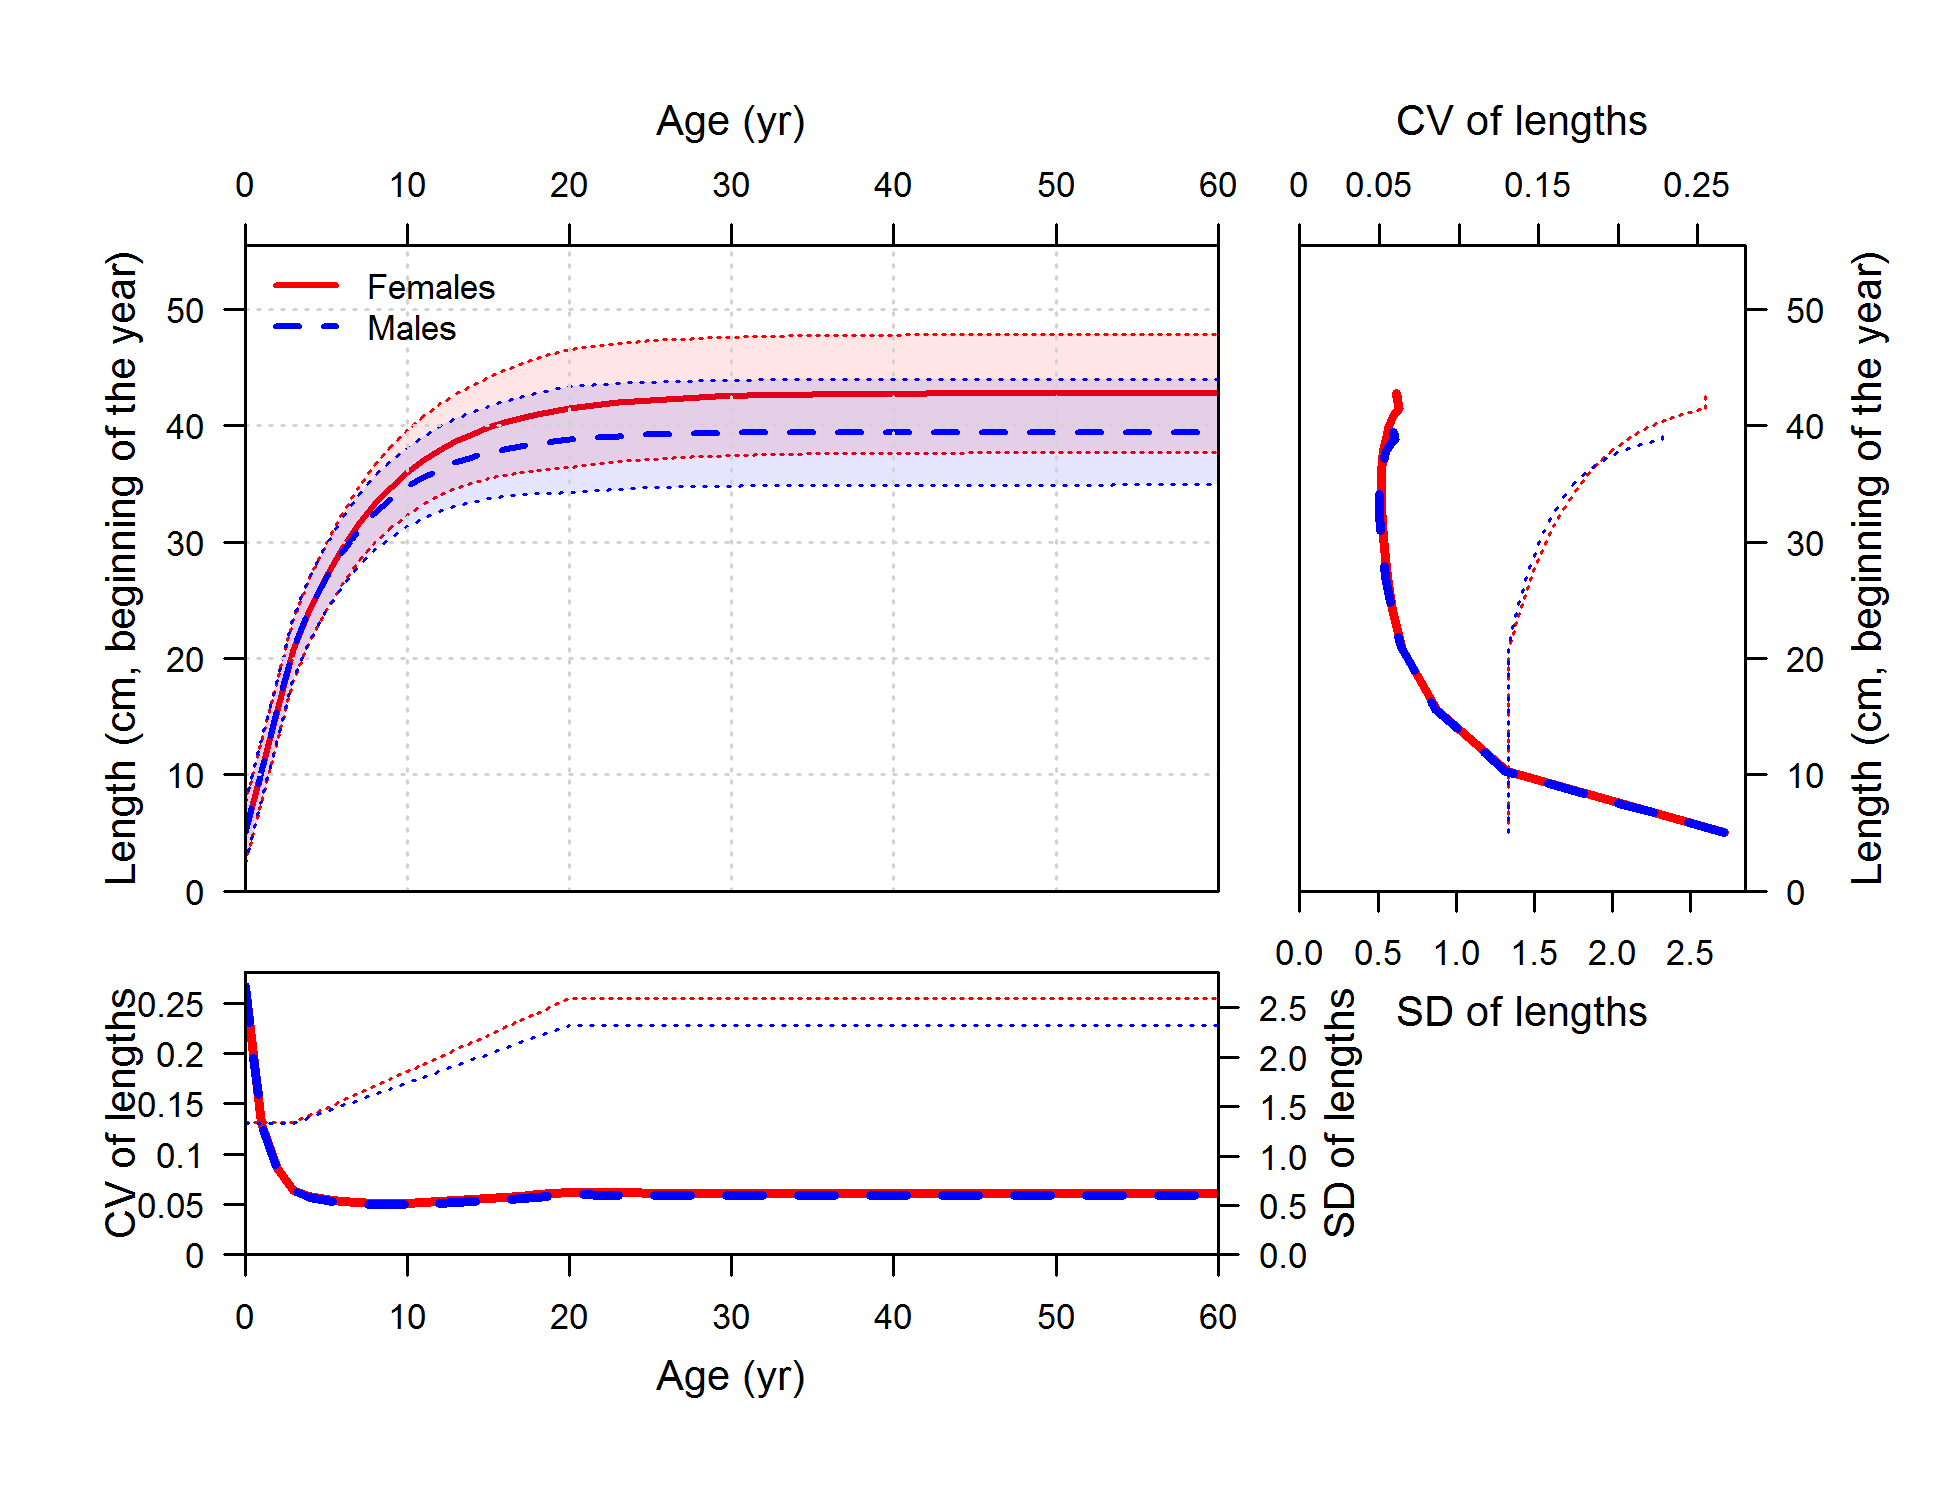
\includegraphics[scale = 0.5]{r4ss/bio2_sizeatage_plus_CV_and_SD.png}
  \end{center}
\end{frame}


\subsection{Selectivity \& Retention}  
\begin{frame}{Fleet structure, Retention, and Selectivity}
  \begin{itemize}
    \item Fishery fleet - includes bottom, mid-water trawls, and fixed gears
      \begin{itemize}
        \item Estimated retention, double-normal selectivity, asymptotic retention
      \end{itemize}
    \item At-sea hake fishery
      \begin{itemize}
        \item Double-normal selectivity
      \end{itemize}
    \item Foreign fleet
      \begin{itemize}
        \item Double-normal selectivity - mirrored to the fishery fleet
      \end{itemize}
    \item Pacific ocean perch survey
      \begin{itemize}
        \item Logistic selectivity 
      \end{itemize}
    \item Triennial shelf survey
      \begin{itemize}
        \item Double normal selectivity 
      \end{itemize}
    \item AFSC slope survey
        \begin{itemize}
        \item Double normal selectivity 
      \end{itemize}
    \item NWFSC slope survey
      \begin{itemize}
        \item Double normal selectivity 
      \end{itemize}
    \item NWFSC shelf-slope survey
      \begin{itemize}
        \item Double normal selectivity 
      \end{itemize}
  \end{itemize}
\end{frame}

\begin{frame}{Selectivity}
  \begin{center}
    \includegraphics[scale = 0.40]{r4ss/POP_selectivity.png}
  \end{center}
\end{frame}

\begin{frame}{Fishery Retention}
\begin{columns}
  \begin{column}{0.4\textwidth}
      Sensitivities to 1992 discard rate
      \begin{itemize}
        \item Low - Removed block  
          \begin{itemize}
            \item $< 0.5\%$ increase in 2017 stock status
          \end{itemize}
        \item High - Assumed average discard based on 2003-2007 
          \begin{itemize}
            \item $< 0.5\%$ decrease in 2017 stock status
          \end{itemize}
      \end{itemize}
  \end{column}
  
  \begin{column}{0.6\textwidth}
  \begin{center}
    \includegraphics[scale = 0.40]{r4ss/POP_retention.png}
  \end{center}
  \end{column}
\end{columns}
\end{frame}



\subsection{Data Weighting}
\begin{frame}{Base Model Data Weights}
  \begin{itemize}
    \item Base model weighted according to Francis weighting approach
  \end{itemize}
  
  \begin{table}[ht]
  \small
  \centering
  \begin{tabular}{p{1.2in}p{0.5in}p{0.5in}p{0.5in}p{0.5in}}
  Fleet & Data & Weight & Data & Weight \\ 
  \hline
  Fishery           & Length &  0.09  & Age & 0.22\\
  At-sea hake       & Length &  0.09  & Age & 0.03\\
  POP survey        & Length &  1.00* & Age & 1.00*\\
  Triennial         & Length &  0.02  & Age & 0.23\\
  AFSC slope        & Length &  0.08  & Age &    -\\
  NWFSC slope       & Length &  0.59  & Age & 0.32\\
  NWFSC shelf-slope & Length &  0.03  & Age & 0.41\\
  \hline
  \end{tabular}
  \end{table}
  * The Francis method suggested upweighting data from the Pacific ocean perch survey to values $> 1$. 
\end{frame}


%---------------------------------------------------------------------------------
\section{Fits to the Data}
%---------------------------------------------------------------------------------
\subsection{Removals}
\begin{frame}{Fit to Discard Rates}
  \begin{center}
    \includegraphics[scale = 0.40, trim={0cm 0cm 0cm 1cm}, clip]{r4ss/POP_discard_fits.png}
  \end{center}
\end{frame}

\begin{frame}{Landings and Estimated Discards}
\begin{columns}
  \begin{column}{0.4\textwidth}
    \begin{itemize}
      \item Estimated discards contributes 3.3\% of the total mortality across all years from the fishery.
    \end{itemize}
  \end{column}
  
  \begin{column}{0.6\textwidth}
  \begin{center}
    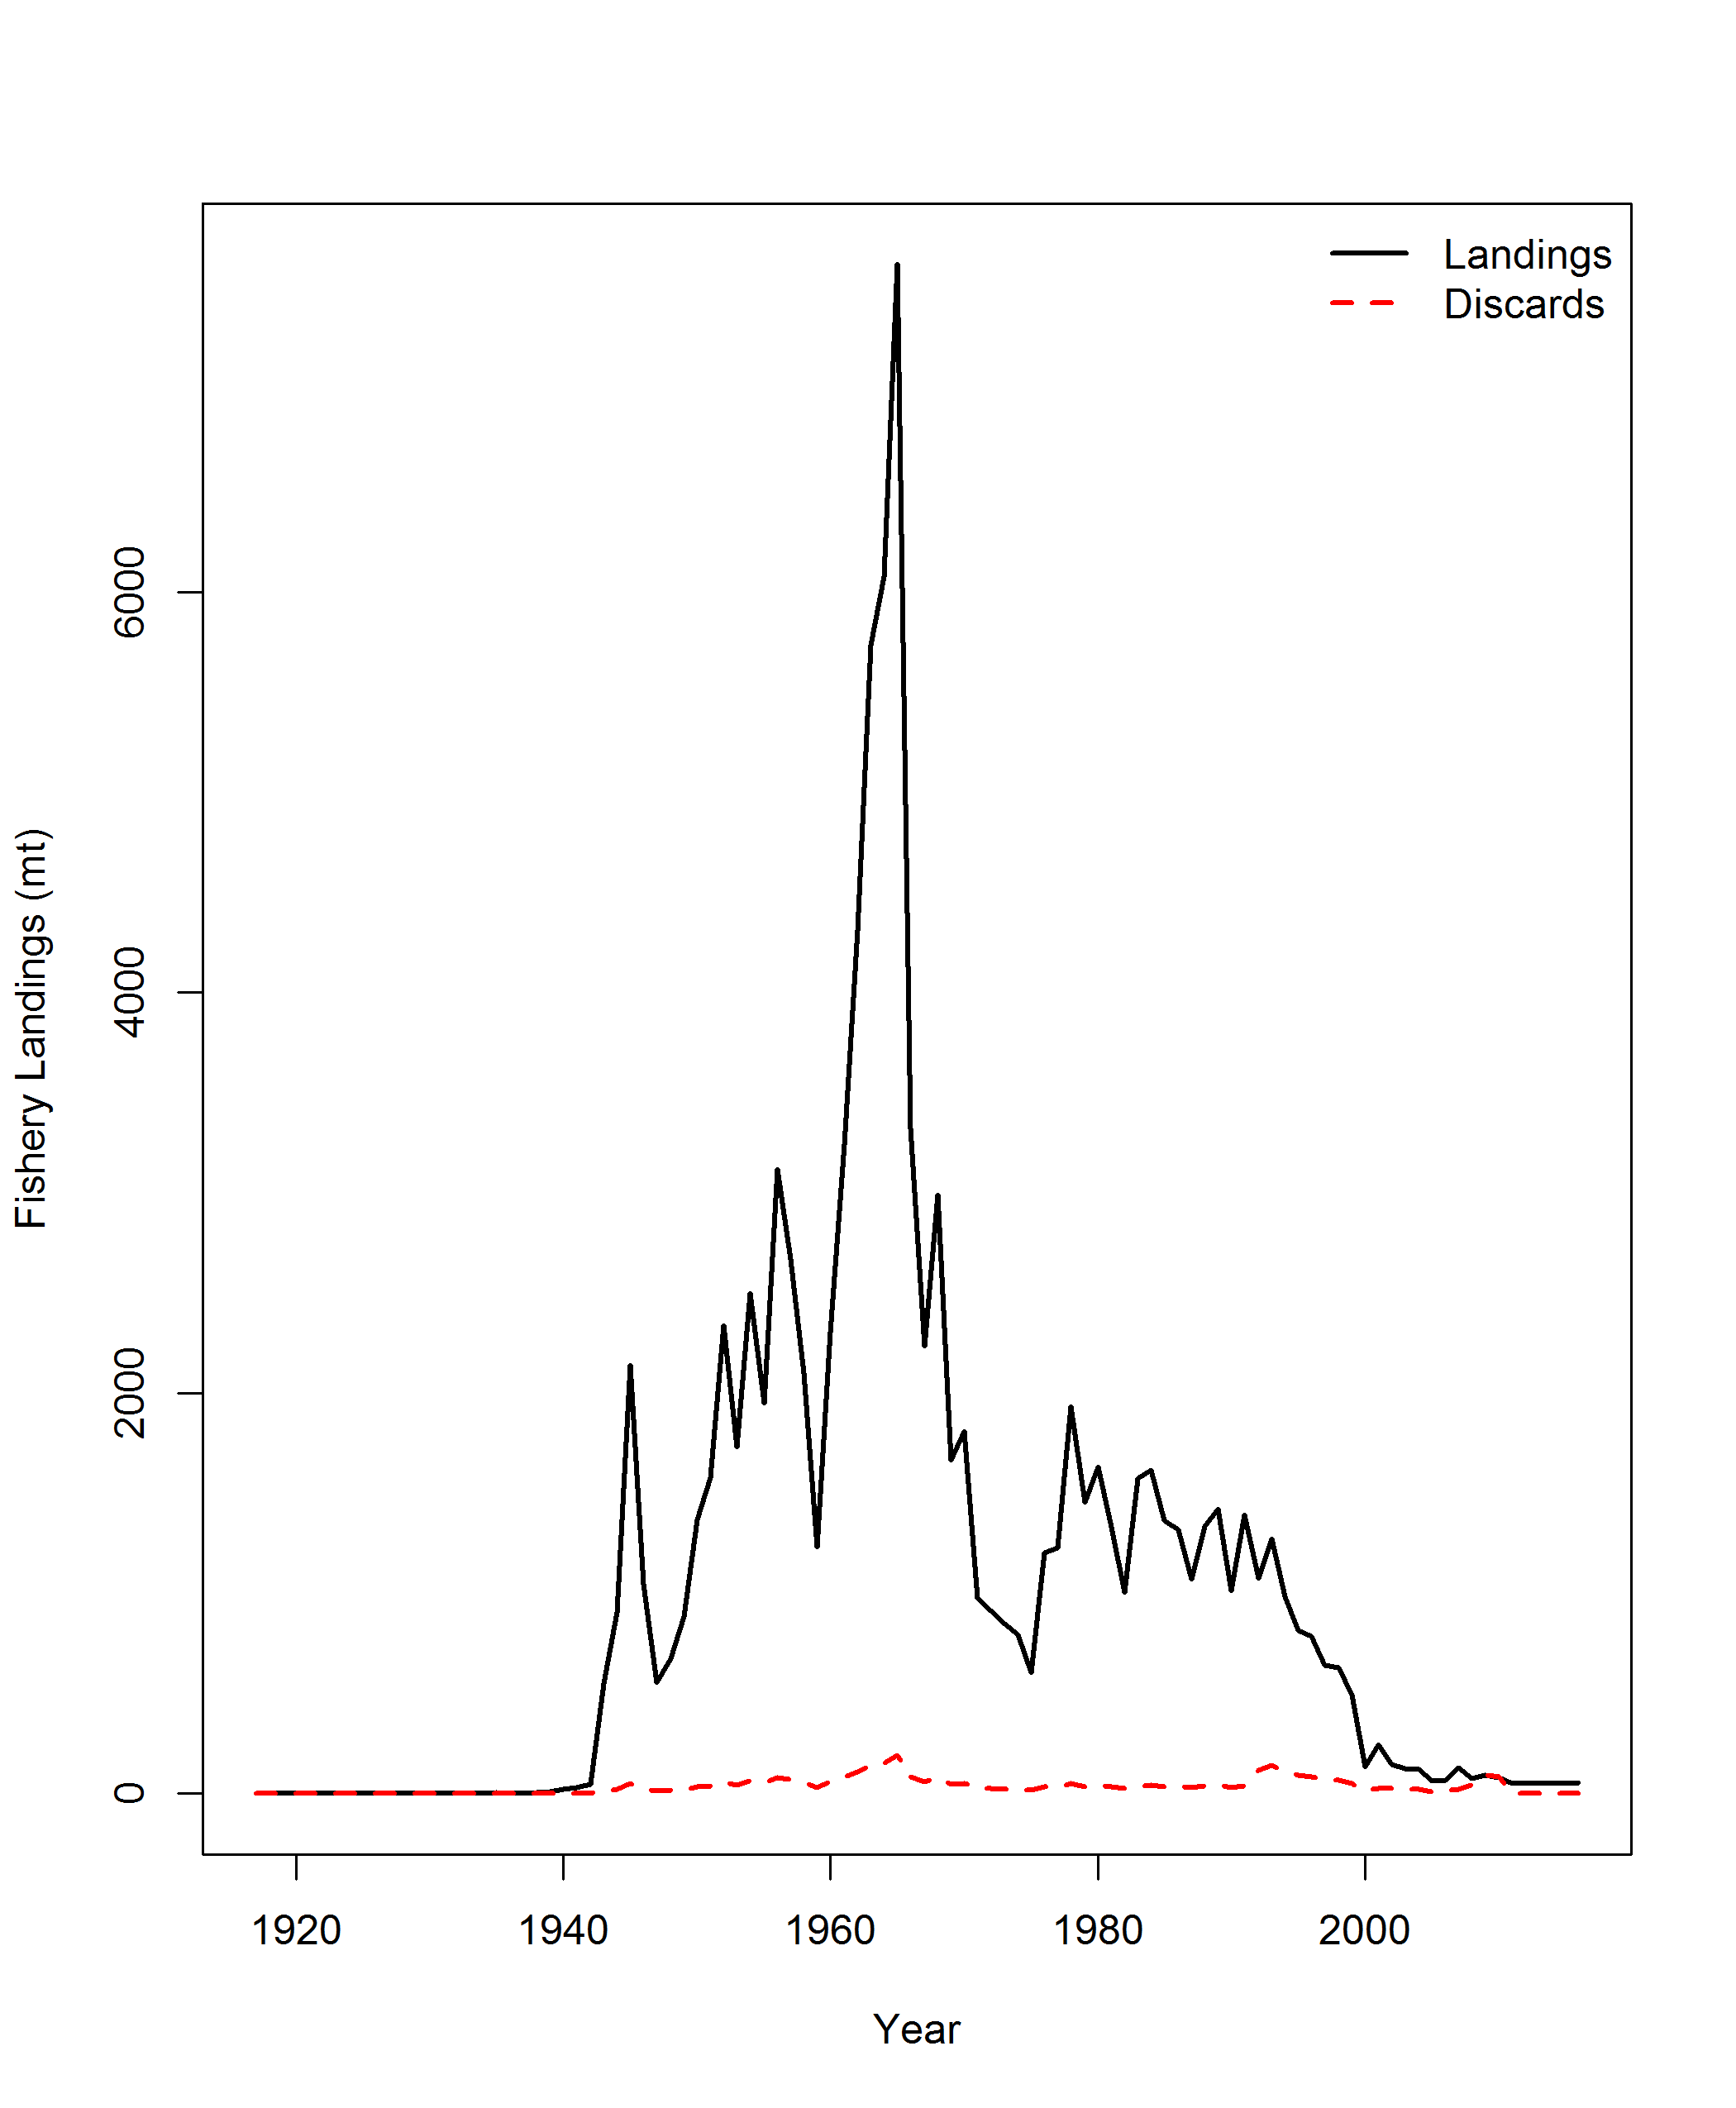
\includegraphics[scale = 0.33]{figures/POP_Landings_Discards.png}
  \end{center}
  \end{column}
\end{columns}
\end{frame}

\subsection{Indices}
\begin{frame}{Added Standard Error for Indices}
  \begin{itemize}
    \item Additional variance was explored for each index of abundance and the CPUE time-series.
    \item Only the Triennial shelf and the NWFSC shelf-slope indices required added variance to allow for model fitting.
      \begin{itemize}
        \item Triennial shelf = 0.390
        \item NWFSC shelf-slope = 0.027 
      \end{itemize}
  \end{itemize}
\end{frame}


\begin{frame}{Fit to the Indices}
  \begin{center}
    \includegraphics[scale = 0.6]{r4ss/POP_index_fits_alt.png}
  \end{center}
\end{frame}


\subsection{Composition Data}
\begin{frame}{Fishery: Length and Age Composition}
  \begin{center}
  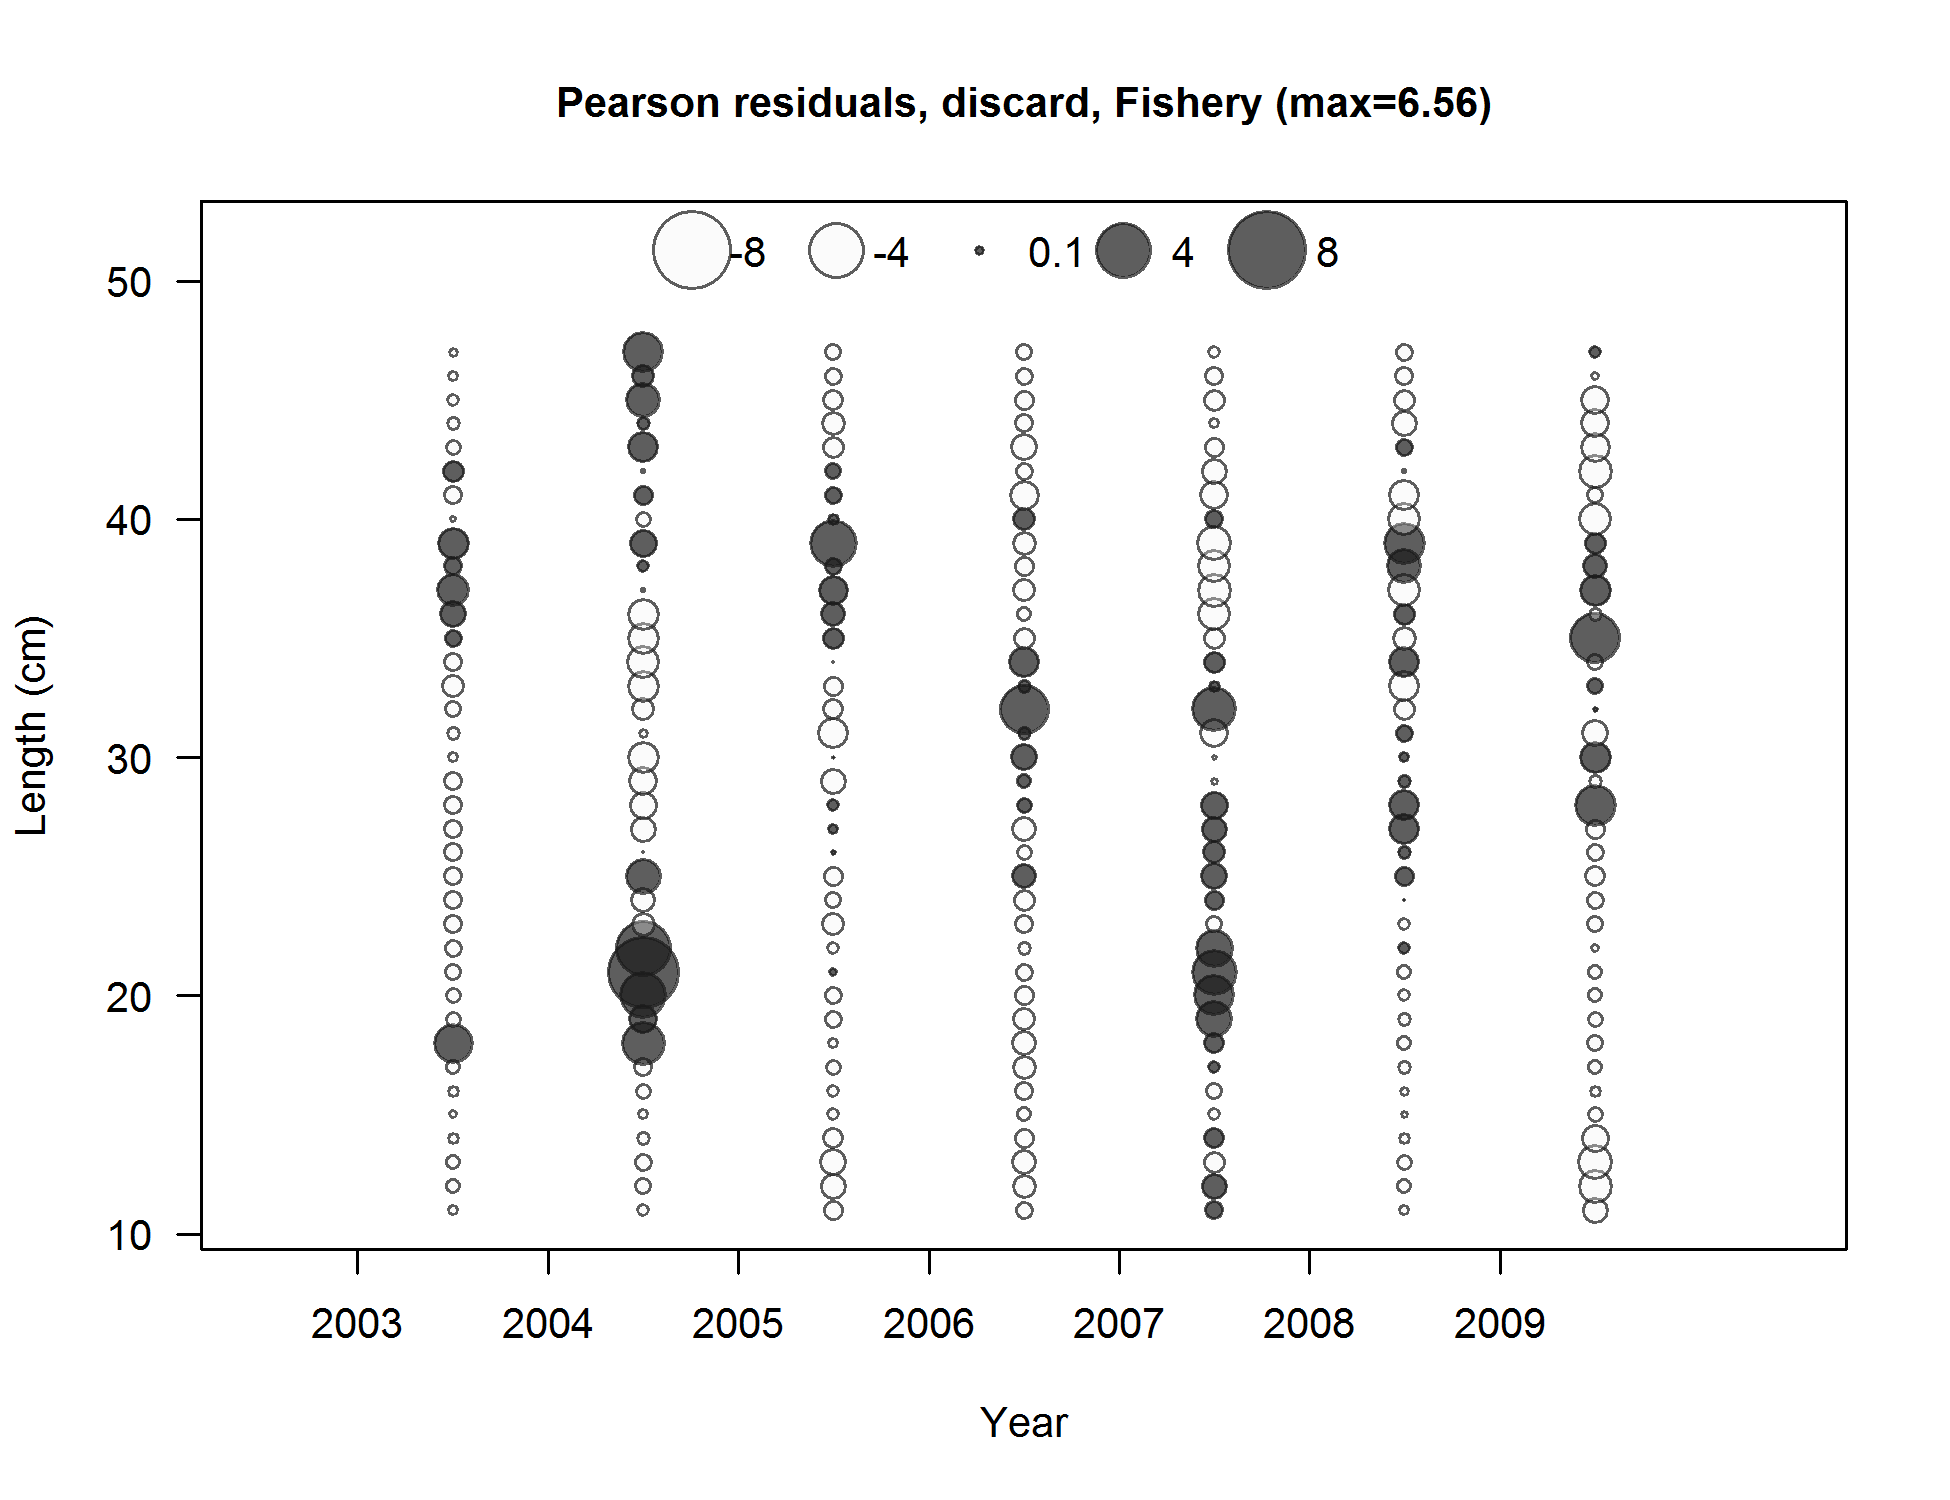
\includegraphics[scale = 0.50]{r4ss/comp_lenfit_residsflt1mkt1.png}
  \end{center}
\end{frame}

\begin{frame}{Fishery: Length and Age Composition}
  \includegraphics[scale = 0.37]{r4ss/comp_lenfit_residsflt1mkt2_page4.png}
  \includegraphics[scale = 0.37]{r4ss/comp_agefit_residsflt1mkt2_page2.png}
\end{frame}

\begin{frame}{Fishery: Mean Length and Age}
  \includegraphics[scale = 0.37]{r4ss/comp_lenfit_data_weighting_TA18_Fishery.png}
  \includegraphics[scale = 0.37]{r4ss/comp_agefit_data_weighting_TA18_Fishery.png}
\end{frame}

\begin{frame}{At-sea hake: Length and Age Composition}
  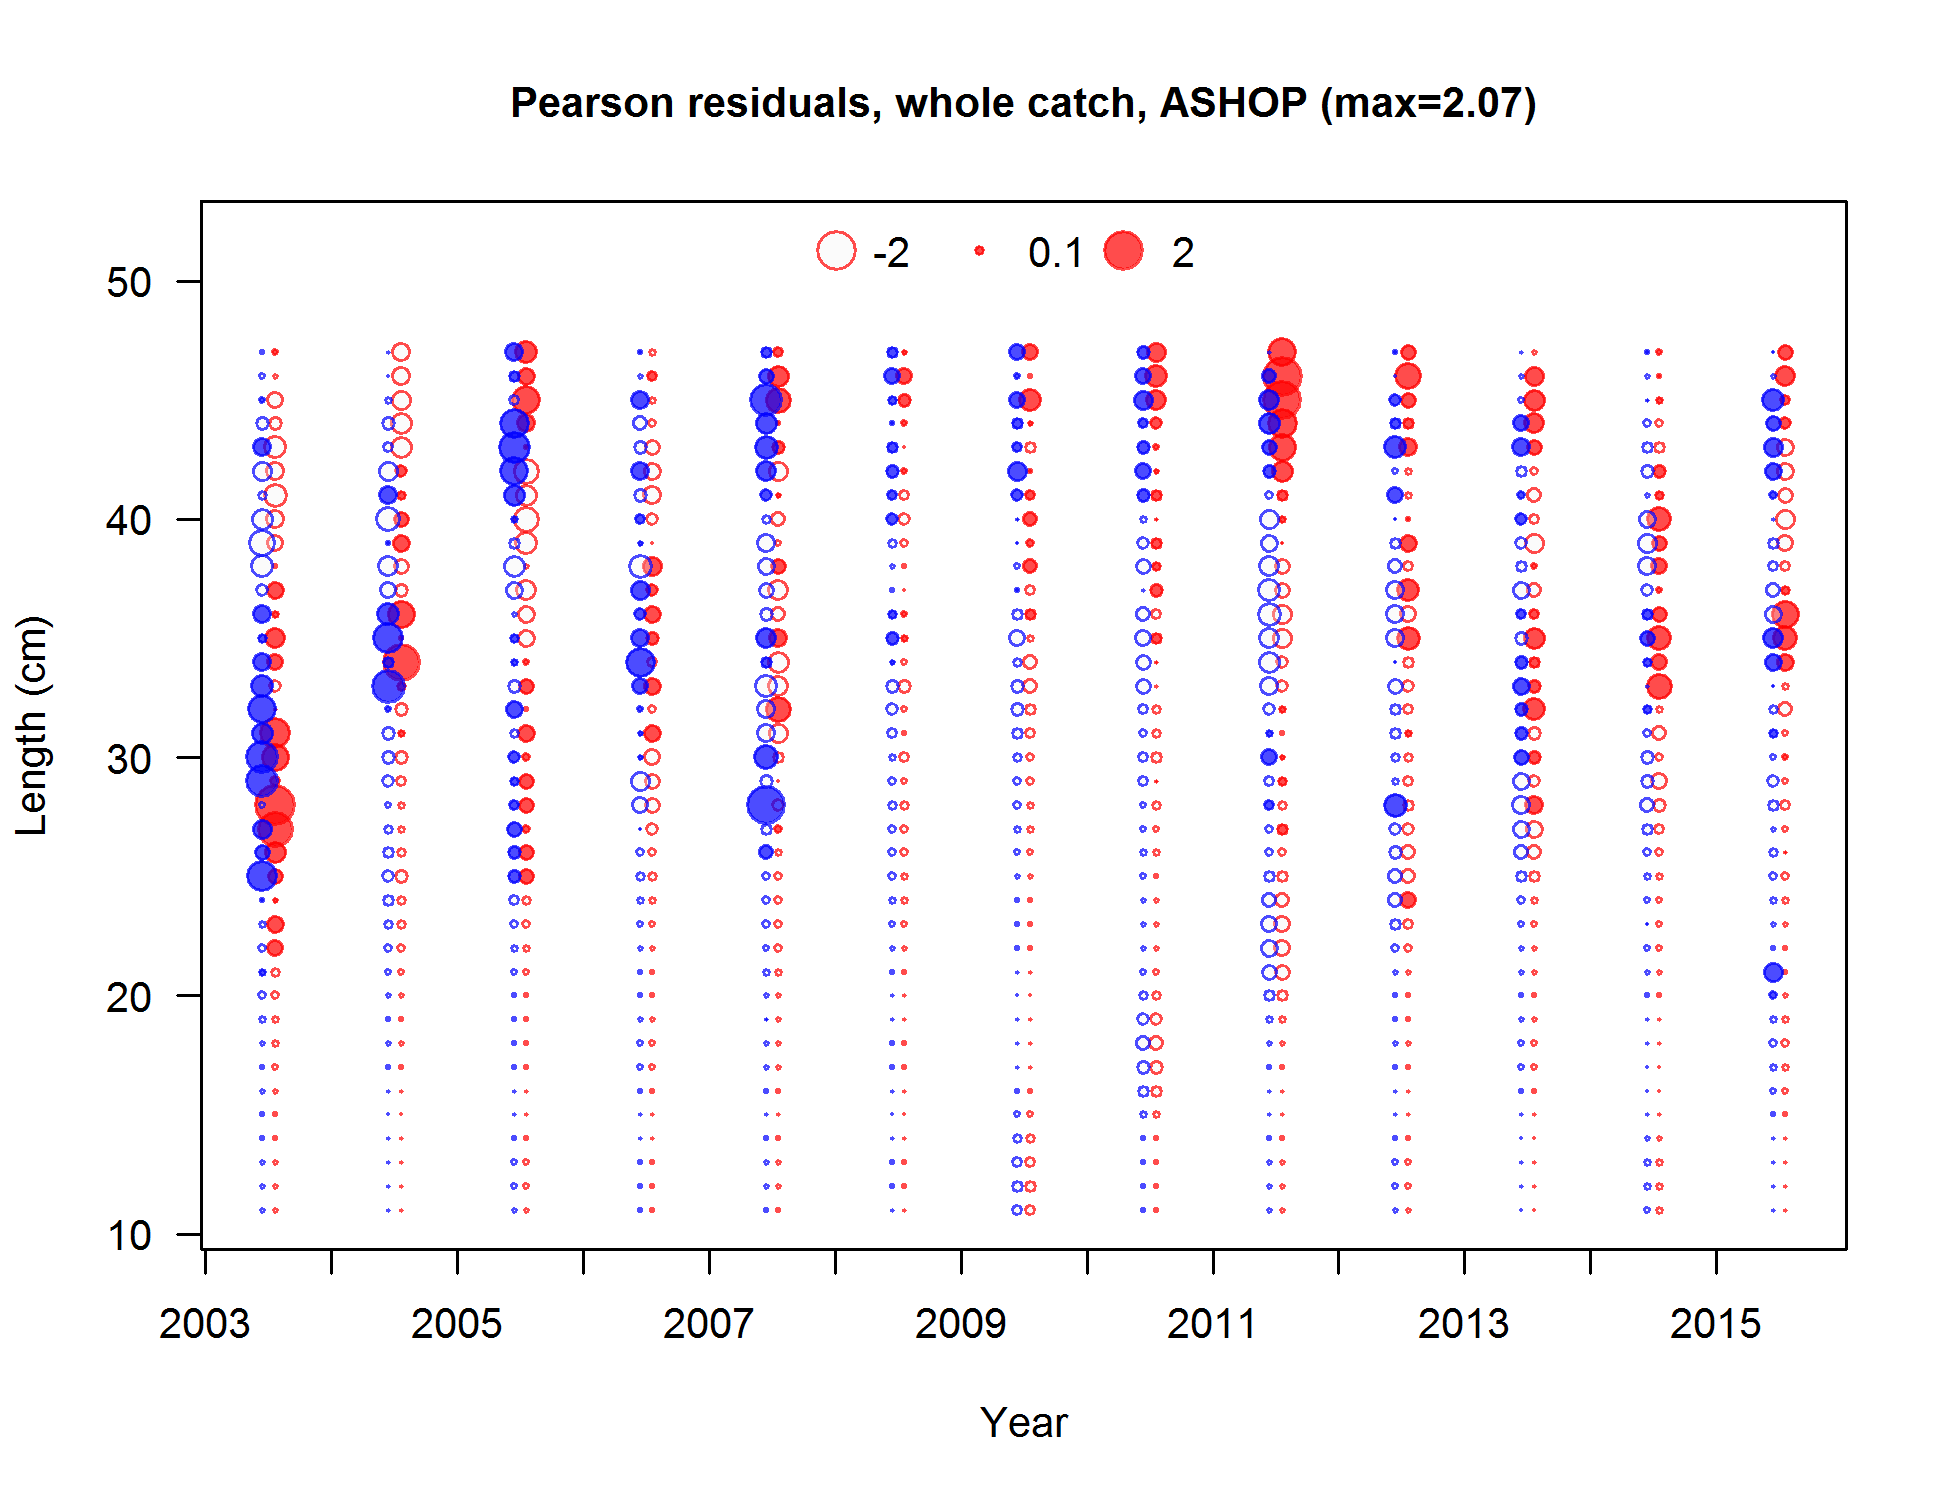
\includegraphics[scale = 0.37]{r4ss/comp_lenfit_residsflt2mkt0.png}
  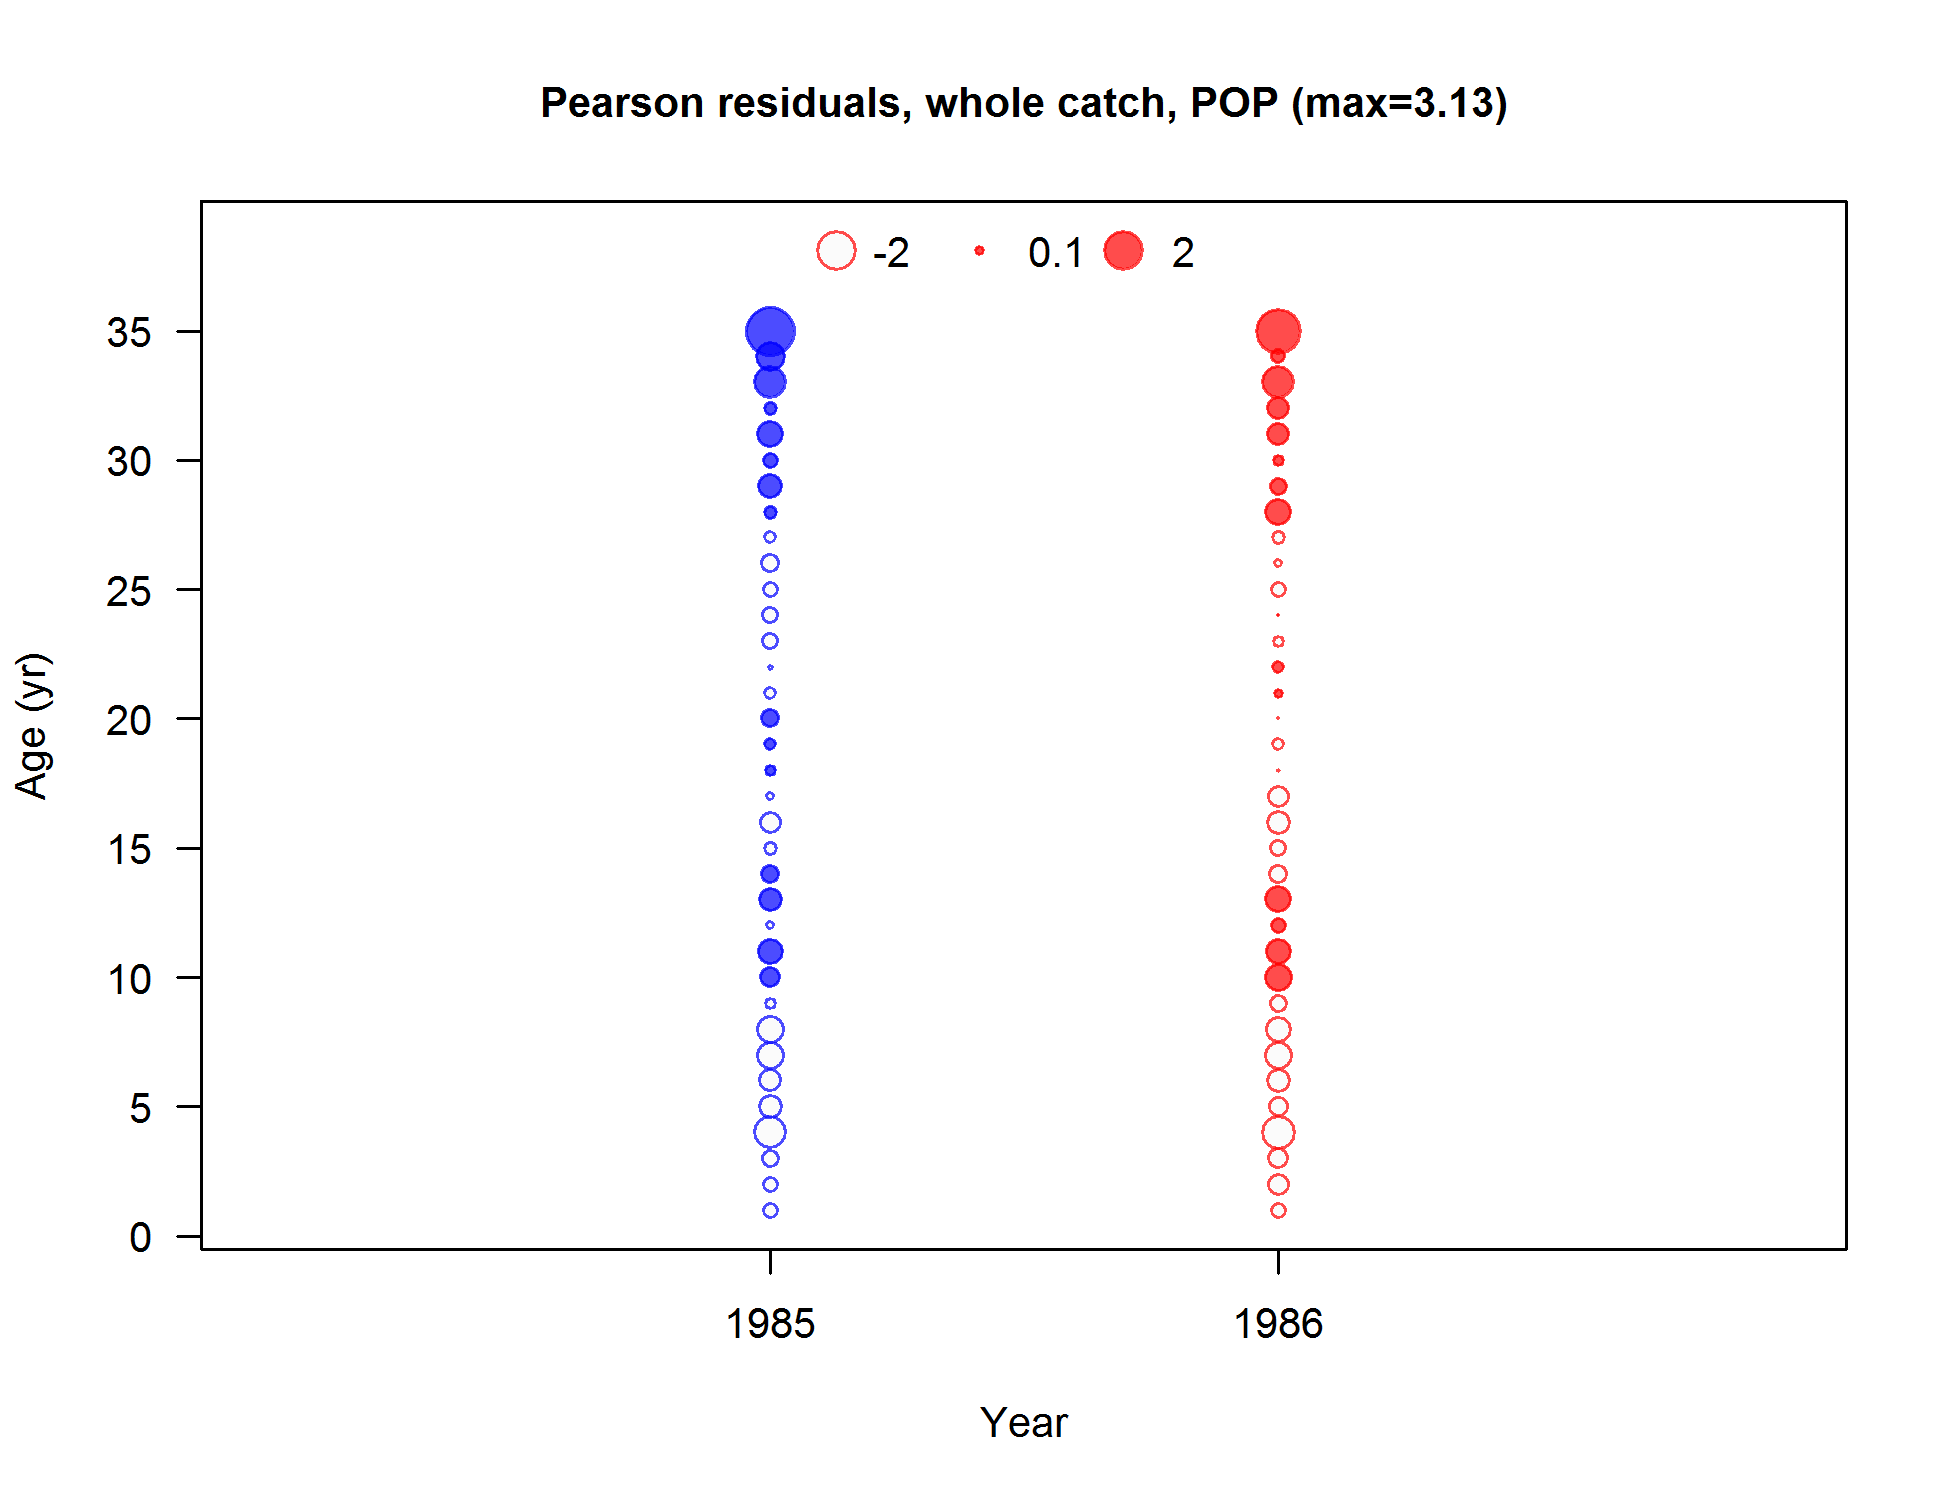
\includegraphics[scale = 0.37]{r4ss/comp_agefit_residsflt2mkt0.png}
\end{frame}

\begin{frame}{At-sea hake: Mean Length and Age}
  \includegraphics[scale = 0.37]{r4ss/comp_lenfit_data_weighting_TA18_At-sea_hake.png}
  \includegraphics[scale = 0.37]{r4ss/comp_agefit_data_weighting_TA18_At-sea_hake.png}
\end{frame}

\begin{frame}{Triennial shelf survey: Length and Age Composition}
  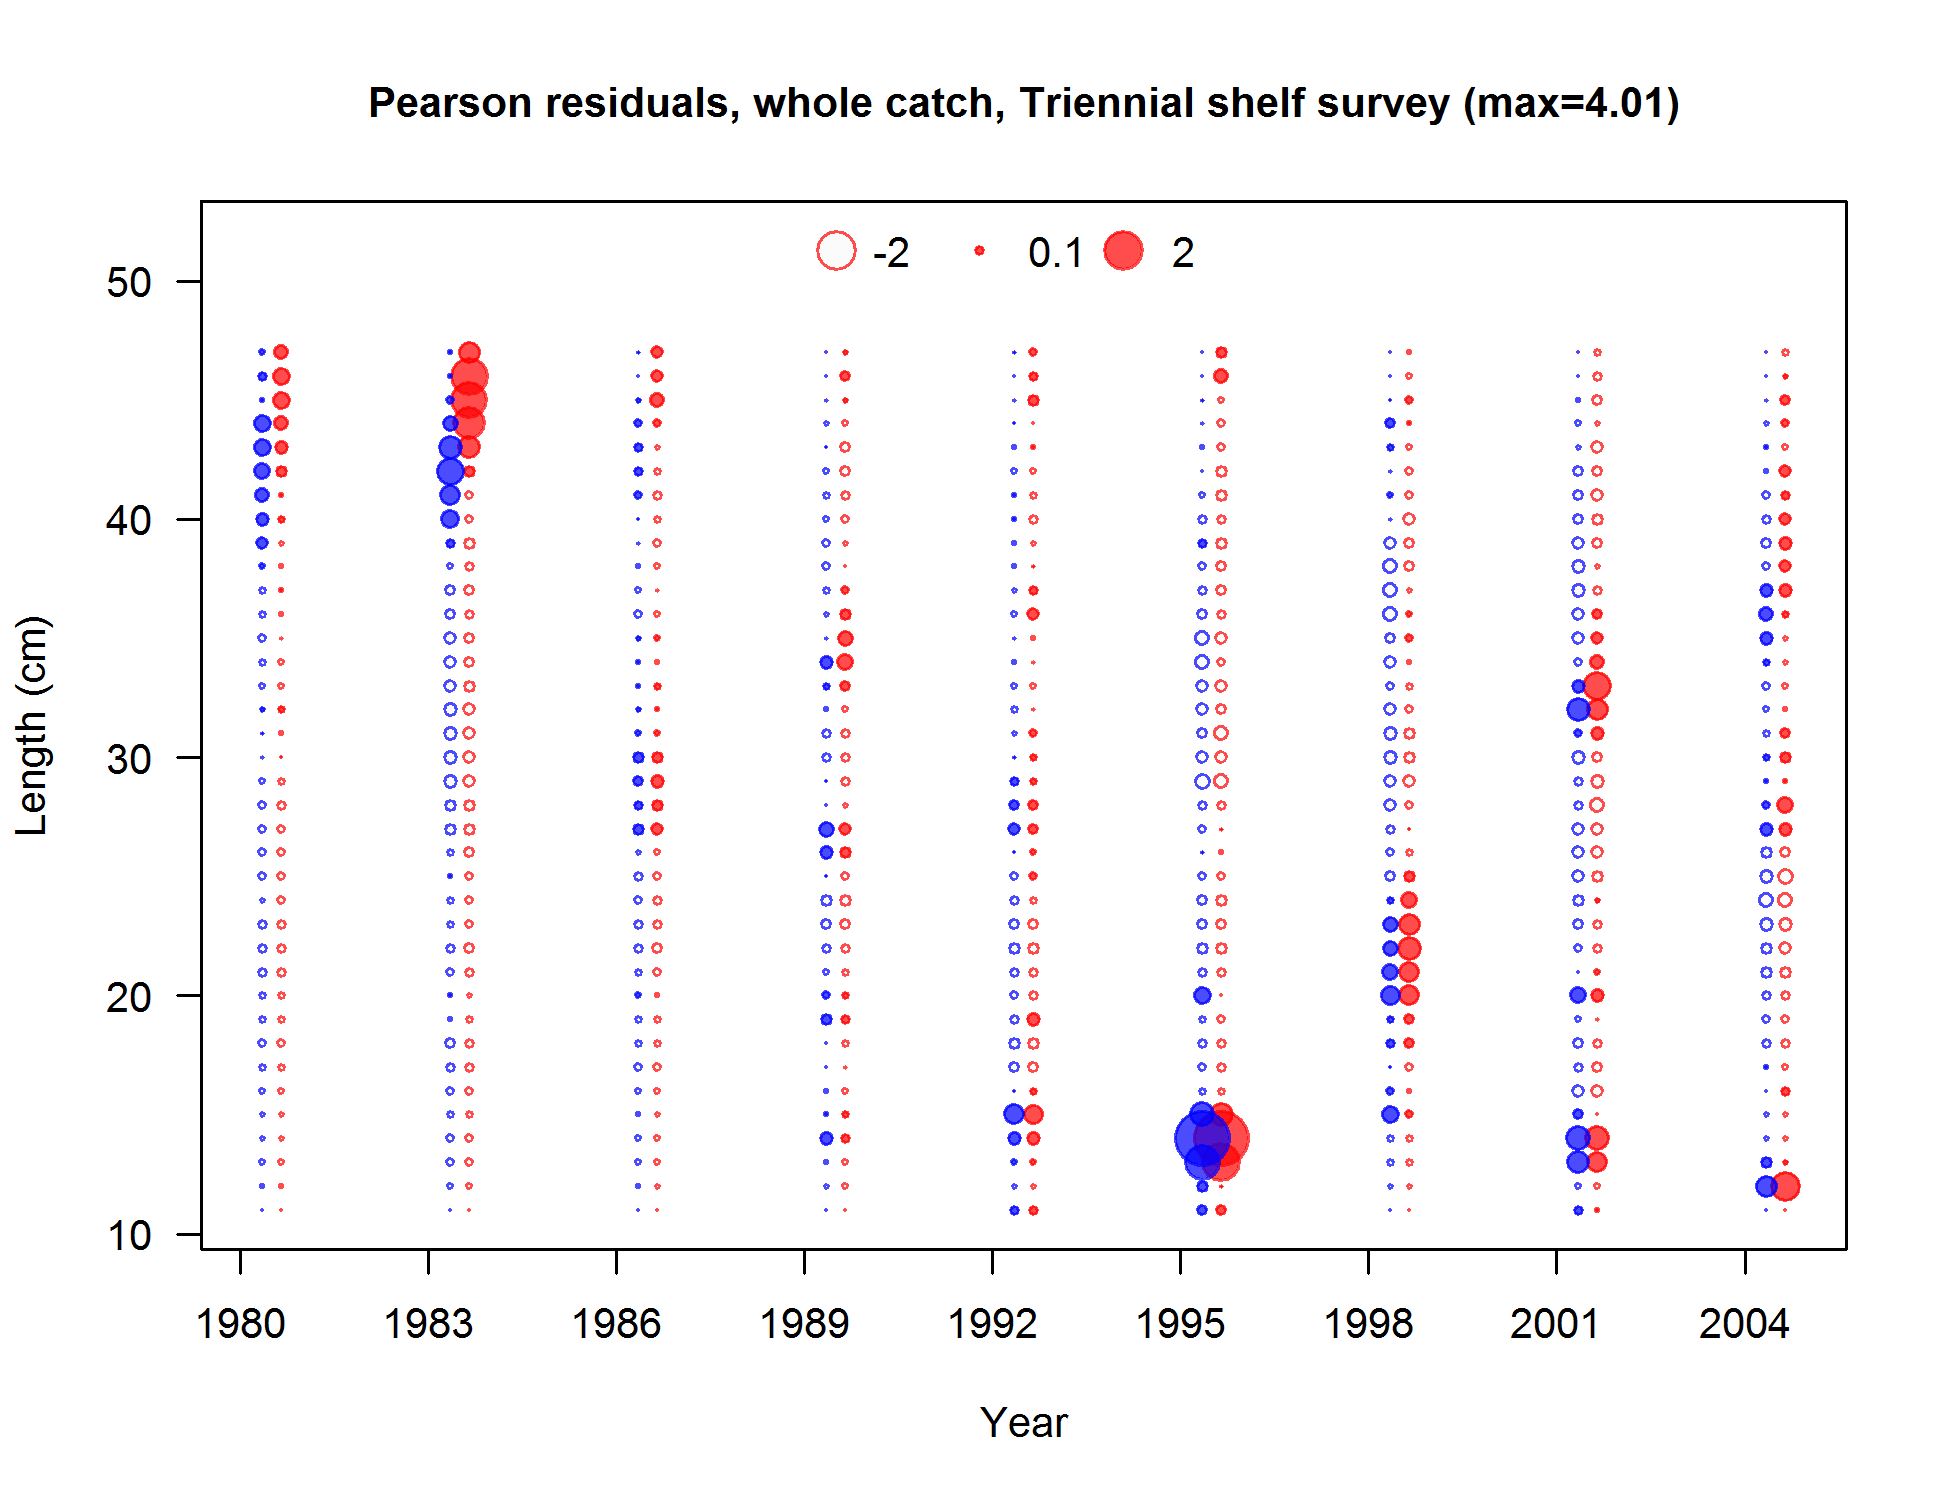
\includegraphics[scale = 0.37]{r4ss/comp_lenfit_residsflt5mkt0.png}
  \includegraphics[scale = 0.37]{r4ss/comp_agefit_residsflt5mkt0.png}
\end{frame}

\begin{frame}{Triennial shelf survey: Mean Length and Age}
  \includegraphics[scale = 0.37]{r4ss/comp_lenfit_data_weighting_TA18_Triennial_shelf_survey.png}
  \includegraphics[scale = 0.37]{r4ss/comp_agefit_data_weighting_TA18_Triennial_shelf_survey.png}
\end{frame}

\begin{frame}{AFSC slope survey: Length Composition}
  \begin{center}
  \includegraphics[scale = 0.50]{r4ss/comp_lenfit_residsflt6mkt0.png}
  \end{center}
\end{frame}

\begin{frame}{AFSC slope survey: Mean Length and Age}
  \begin{center}
  \includegraphics[scale = 0.50]{r4ss/comp_lenfit_data_weighting_TA18_AFSC_slope_survey.png}
  \end{center}
\end{frame}

\begin{frame}{NWFSC slope survey: Length and Age Composition}
  \includegraphics[scale = 0.37]{r4ss/comp_lenfit_residsflt7mkt0.png}
  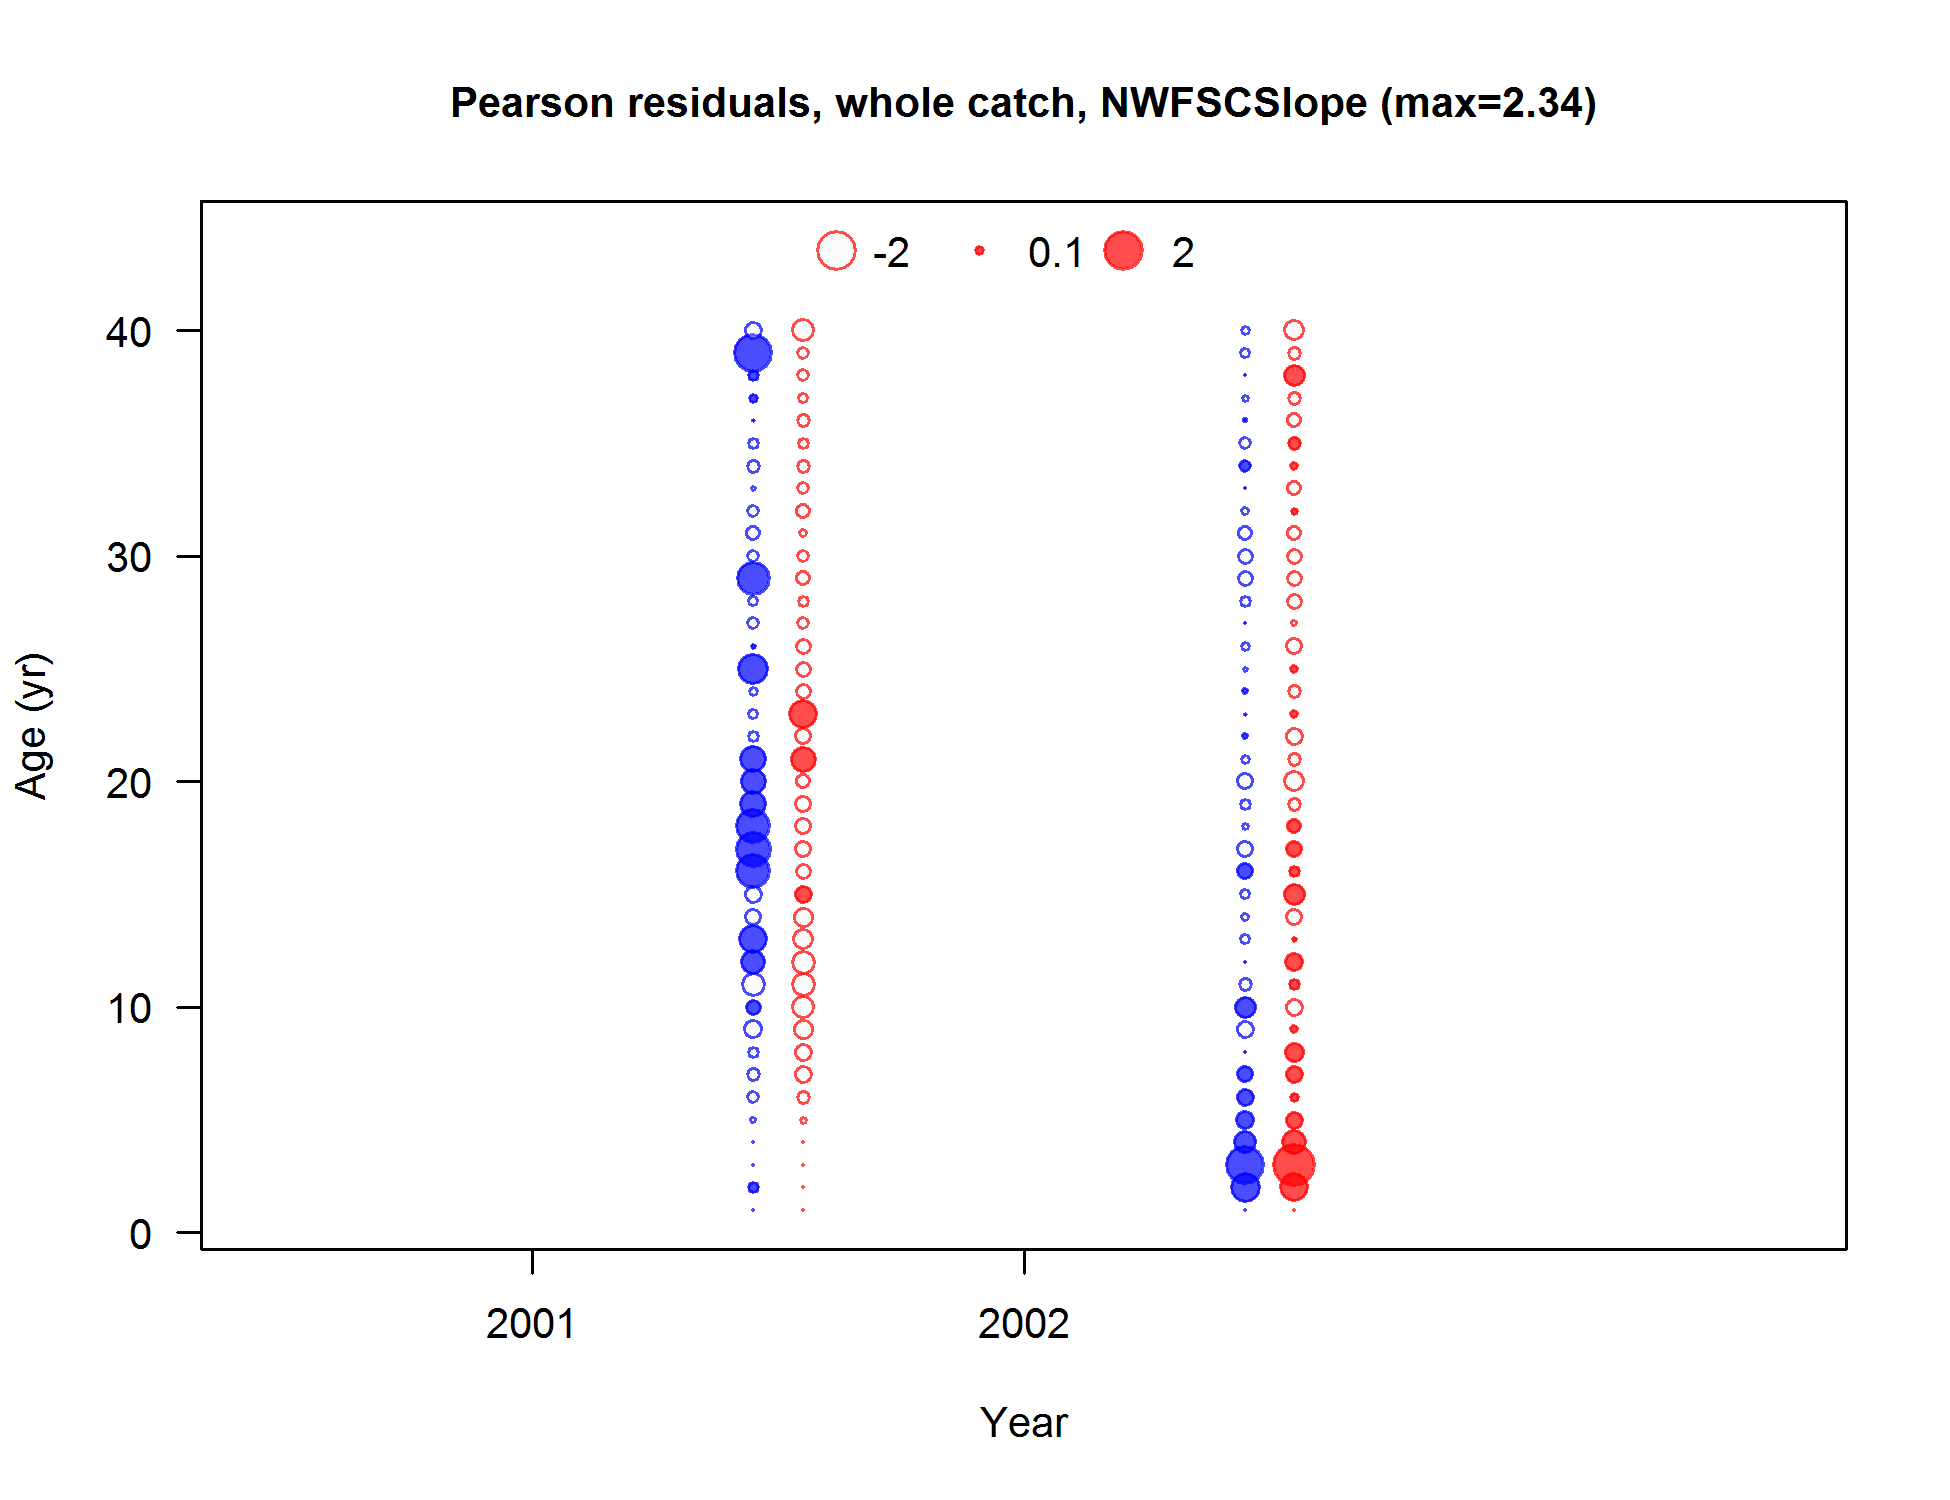
\includegraphics[scale = 0.37]{r4ss/comp_agefit_residsflt7mkt0.png}
\end{frame}

\begin{frame}{NWFSC slope survey: Mean Length and Age}
  \includegraphics[scale = 0.37]{r4ss/comp_lenfit_data_weighting_TA18_NWFSC_slope_survey.png}
  \includegraphics[scale = 0.37]{r4ss/comp_agefit_data_weighting_TA18_NWFSC_slope_survey.png}
\end{frame}

\begin{frame}{NWFSC shelf-slope survey: Length Composition}
  \begin{center}
  \includegraphics[scale = 0.50]{r4ss/comp_lenfit_residsflt8mkt0.png}
  \end{center}
\end{frame}

\begin{frame}{NWFSC shelf-slope survey: Conditional Age-at-Length Composition}
  \includegraphics[scale = 0.37]{r4ss/comp_condAALfit_Andre_plotsflt8mkt0_page1.png}
  \includegraphics[scale = 0.37]{r4ss/comp_condAALfit_Andre_plotsflt8mkt0_page2.png}
\end{frame}

\begin{frame}{NWFSC shelf-slope survey: Conditional Age-at-Length Composition}
  \includegraphics[scale = 0.37]{r4ss/comp_condAALfit_Andre_plotsflt8mkt0_page3.png}
  \includegraphics[scale = 0.37]{r4ss/comp_condAALfit_Andre_plotsflt8mkt0_page4.png}
\end{frame}

\begin{frame}{NWFSC shelf-slope survey: Conditional Age-at-Length Composition}
  \begin{center}
  \includegraphics[scale = 0.50]{r4ss/comp_condAALfit_Andre_plotsflt8mkt0_page5.png}
  \end{center}
\end{frame}

\begin{frame}{NWFSC shelf-slope survey: Mean Length and Age}
  \includegraphics[scale = 0.37]{r4ss/comp_lenfit_data_weighting_TA18_NWFSC_shelf-slope_survey.png}
  \includegraphics[scale = 0.37]{r4ss/comp_condAALfit_data_weighting_TA18_condAgeNWFSC_shelf-slope_survey.png}
\end{frame}

\begin{frame}{Aggregated Length and Age Composition Fits}
  \includegraphics[scale = 0.37]{r4ss/comp_lenfit__aggregated_across_time.png}
  \includegraphics[scale = 0.37]{r4ss/comp_agefit__aggregated_across_time.png}
\end{frame}

%---------------------------------------------------------------------------------
\section{Population Estimates}
%---------------------------------------------------------------------------------
\subsection{Size and Scale}
\begin{frame}{Spawning Output}
  \begin{center}
    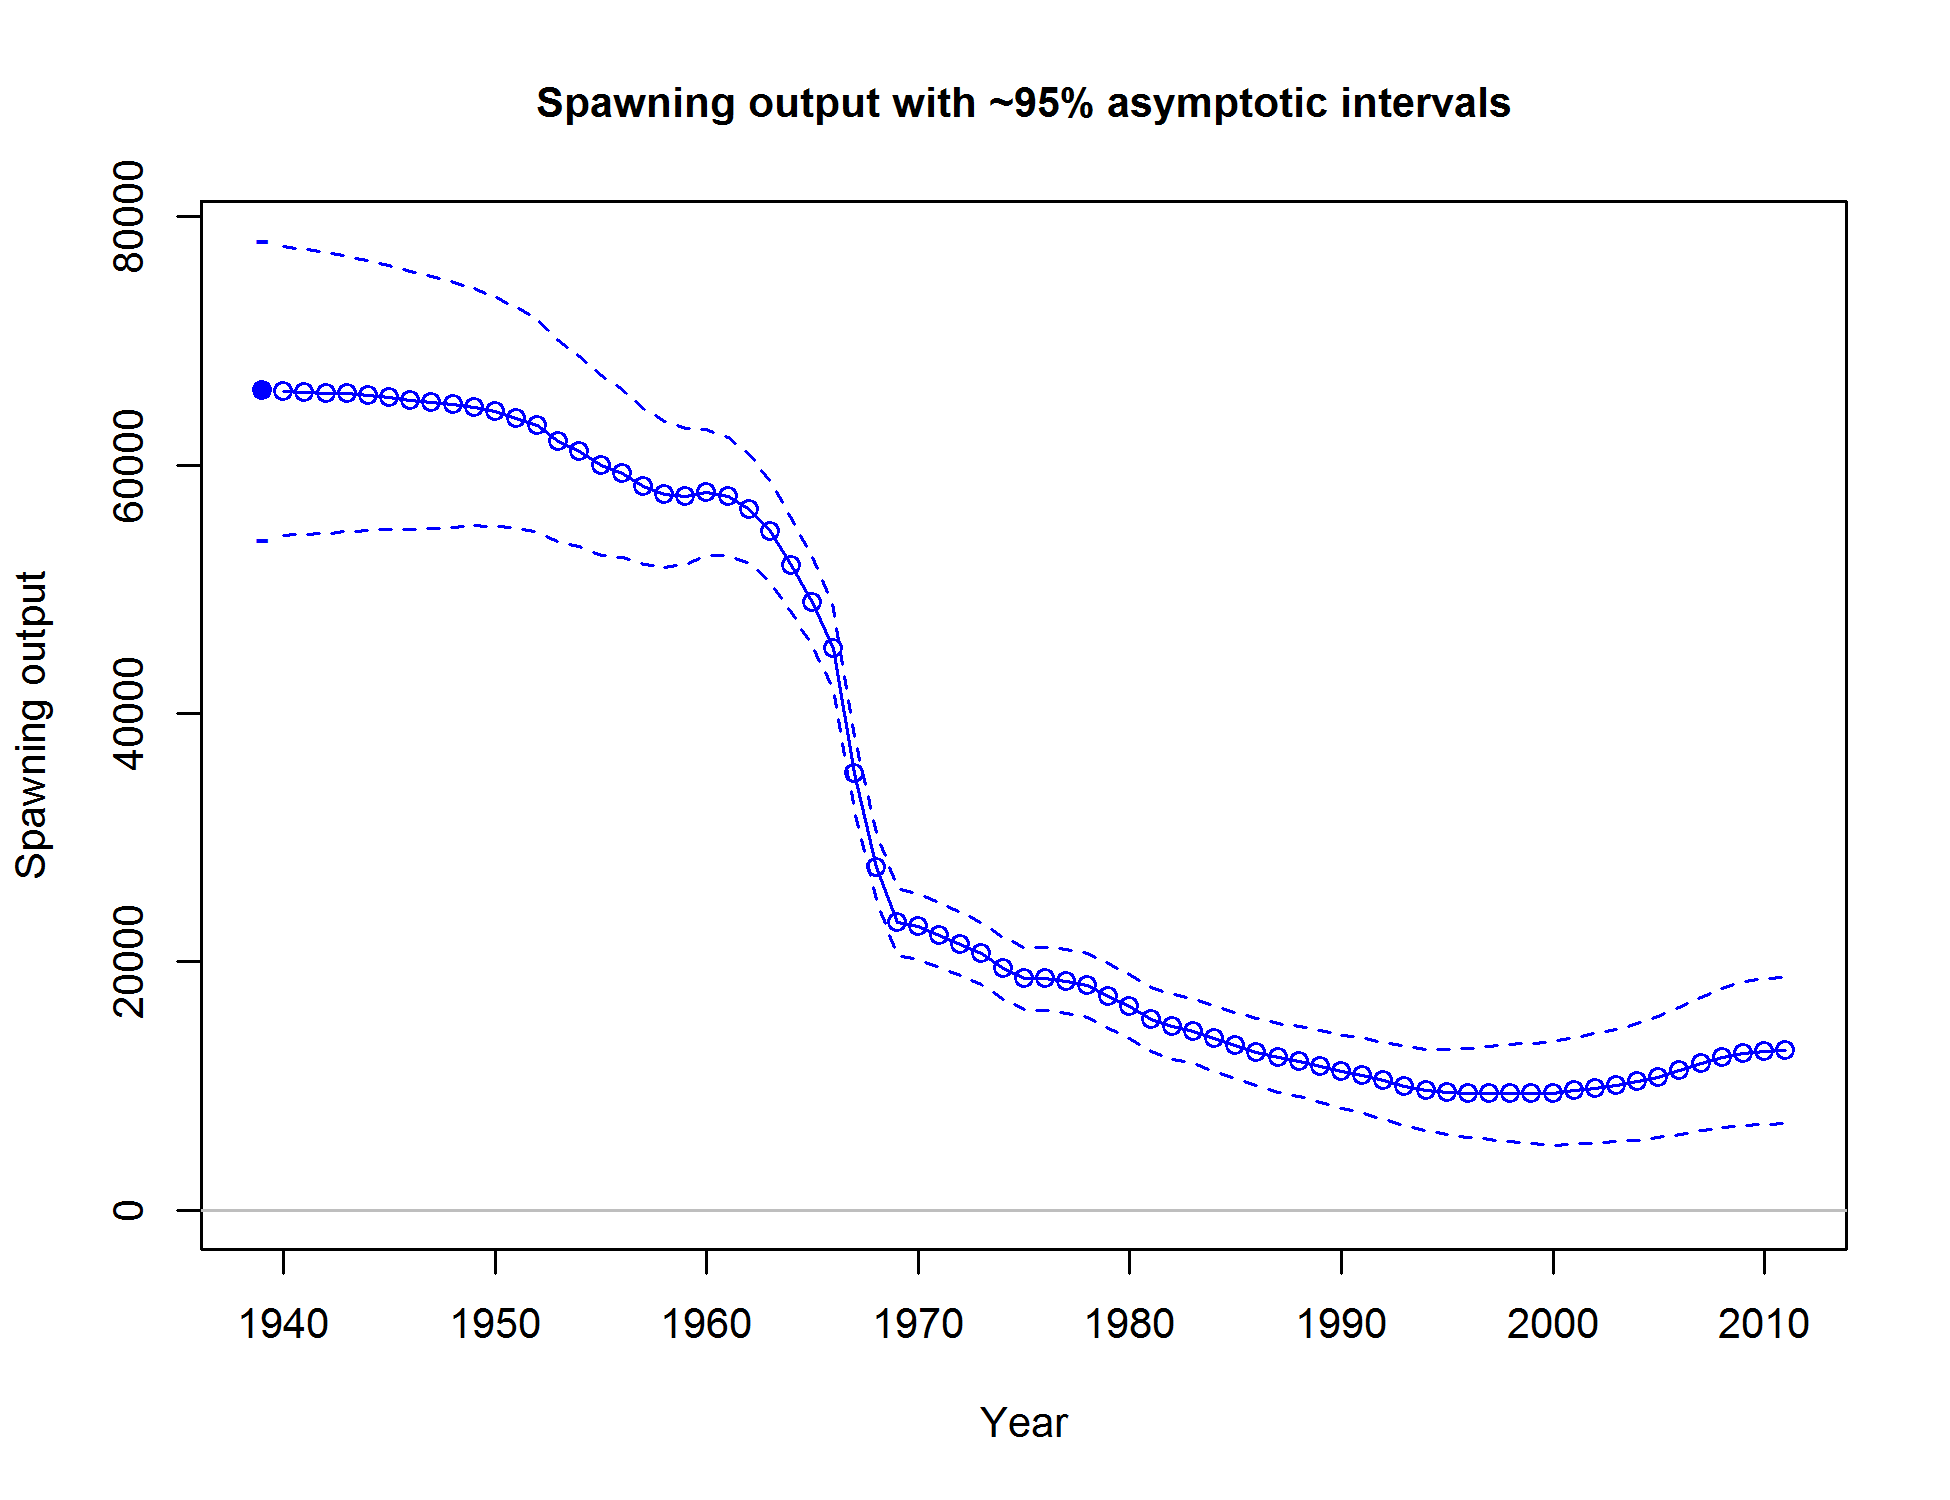
\includegraphics[scale = 0.50]{r4ss/ts7_Spawning_output_with_95_asymptotic_intervals_intervals.png}
  \end{center}
\end{frame}

\begin{frame}{Relative Spawning Output (Depletion)}
  \begin{center}
    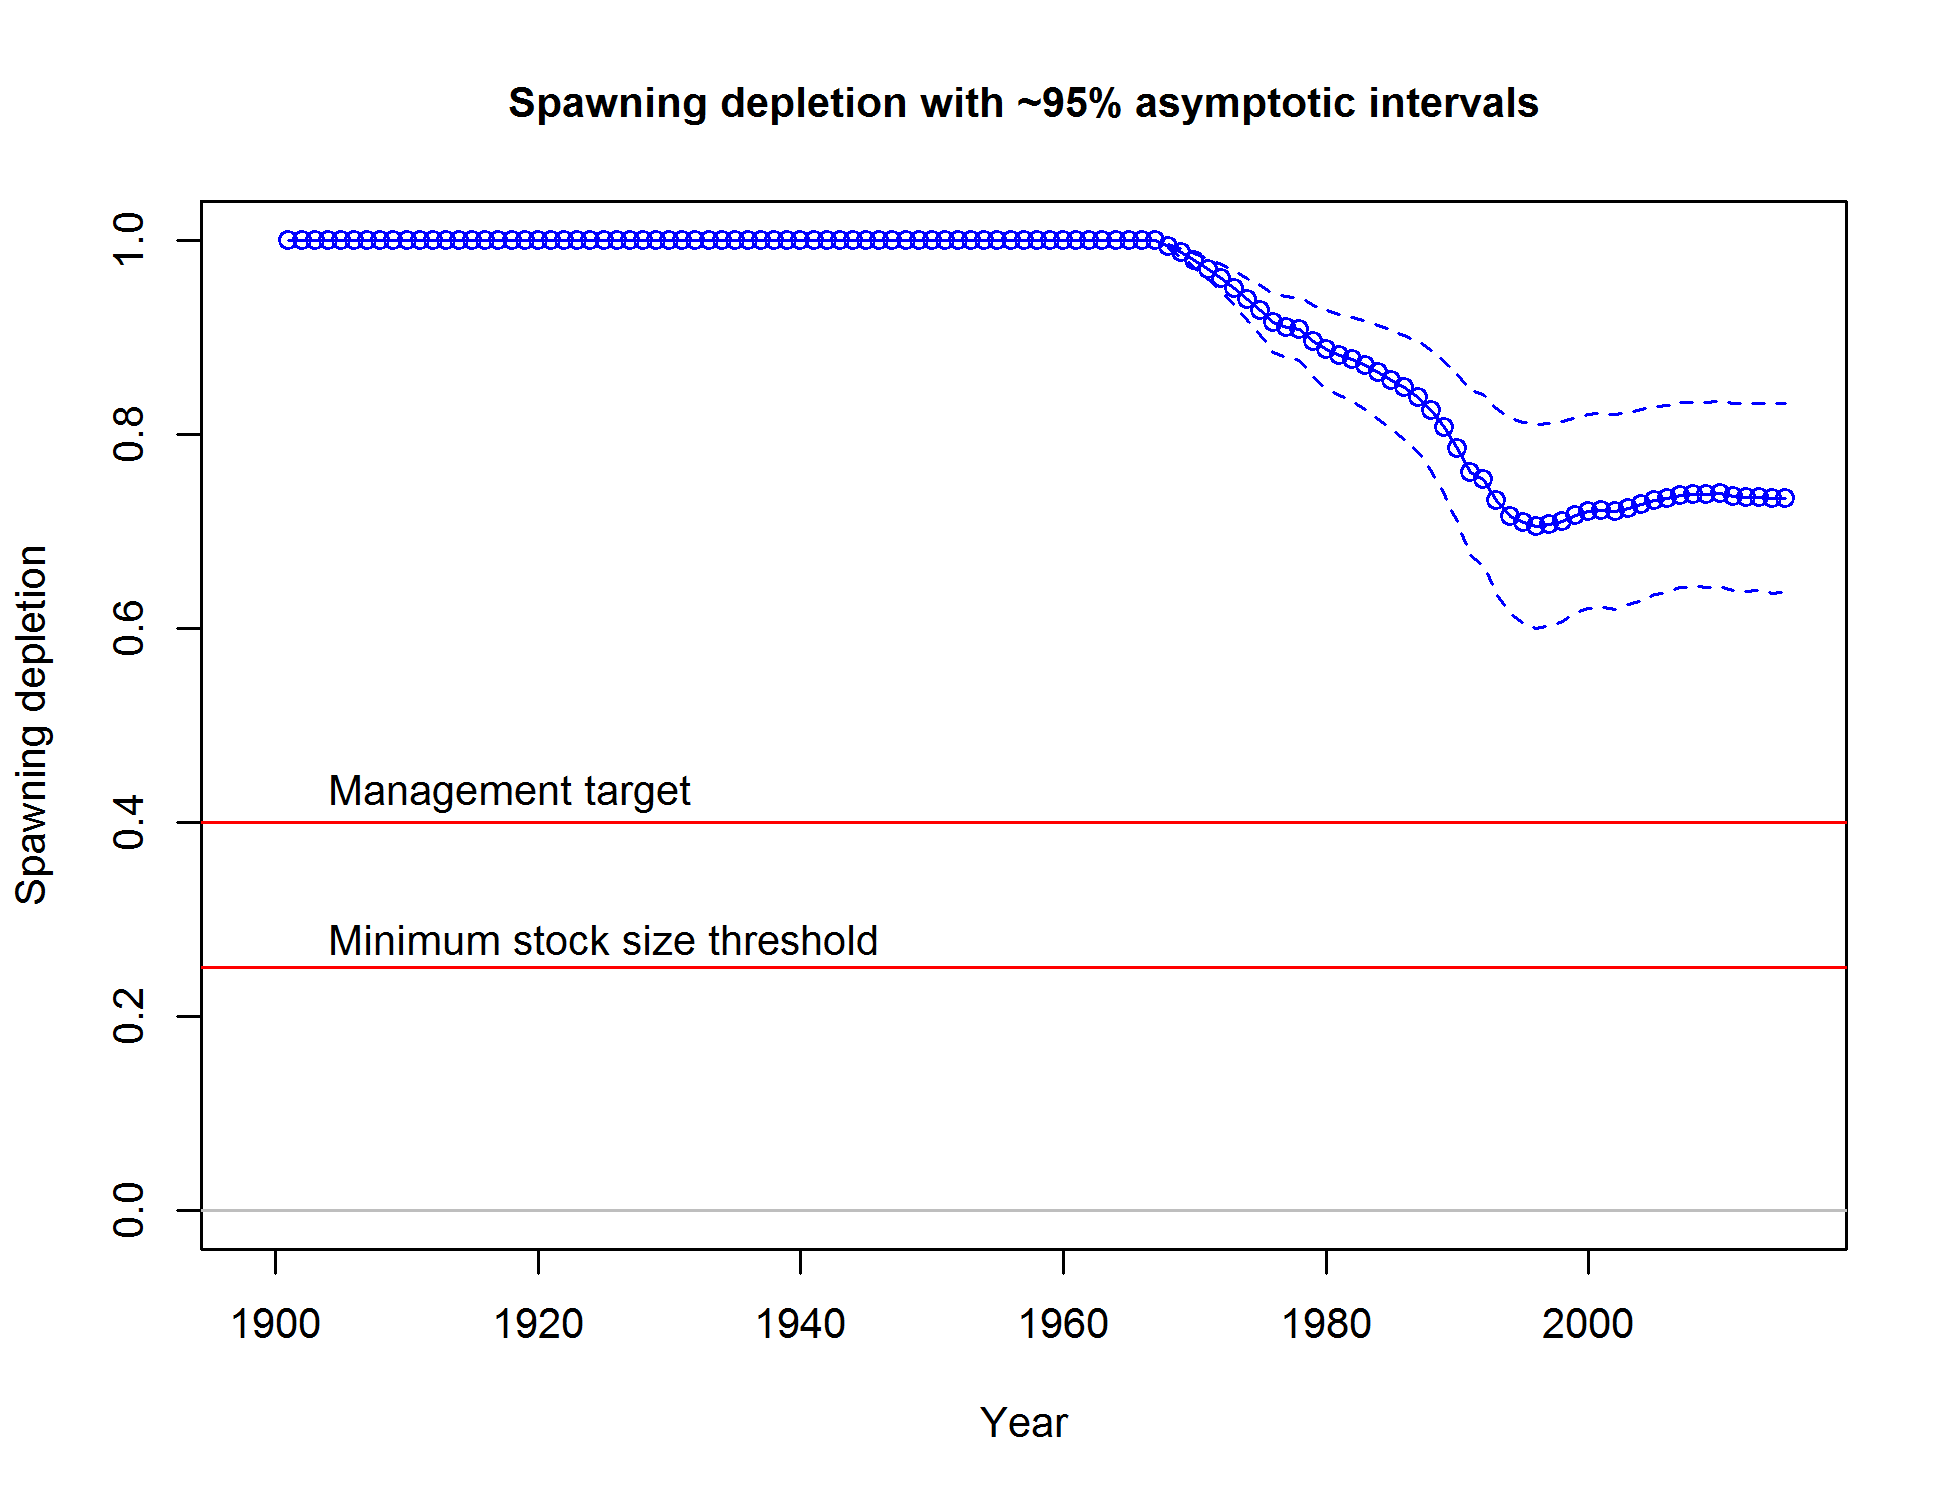
\includegraphics[scale = 0.50]{r4ss/ts9_Spawning_depletion_with_95_asymptotic_intervals_intervals.png}
  \end{center}
  \begin{tikzpicture}[remember picture, overlay, shift = {(current page.center)}]
    \node[black] at (2.75, 1) { 74.9\%};
  \end{tikzpicture}
\end{frame}

\subsection{Recruitment}
\begin{frame}{Estimated Annual Recruitment}
  \begin{center}
    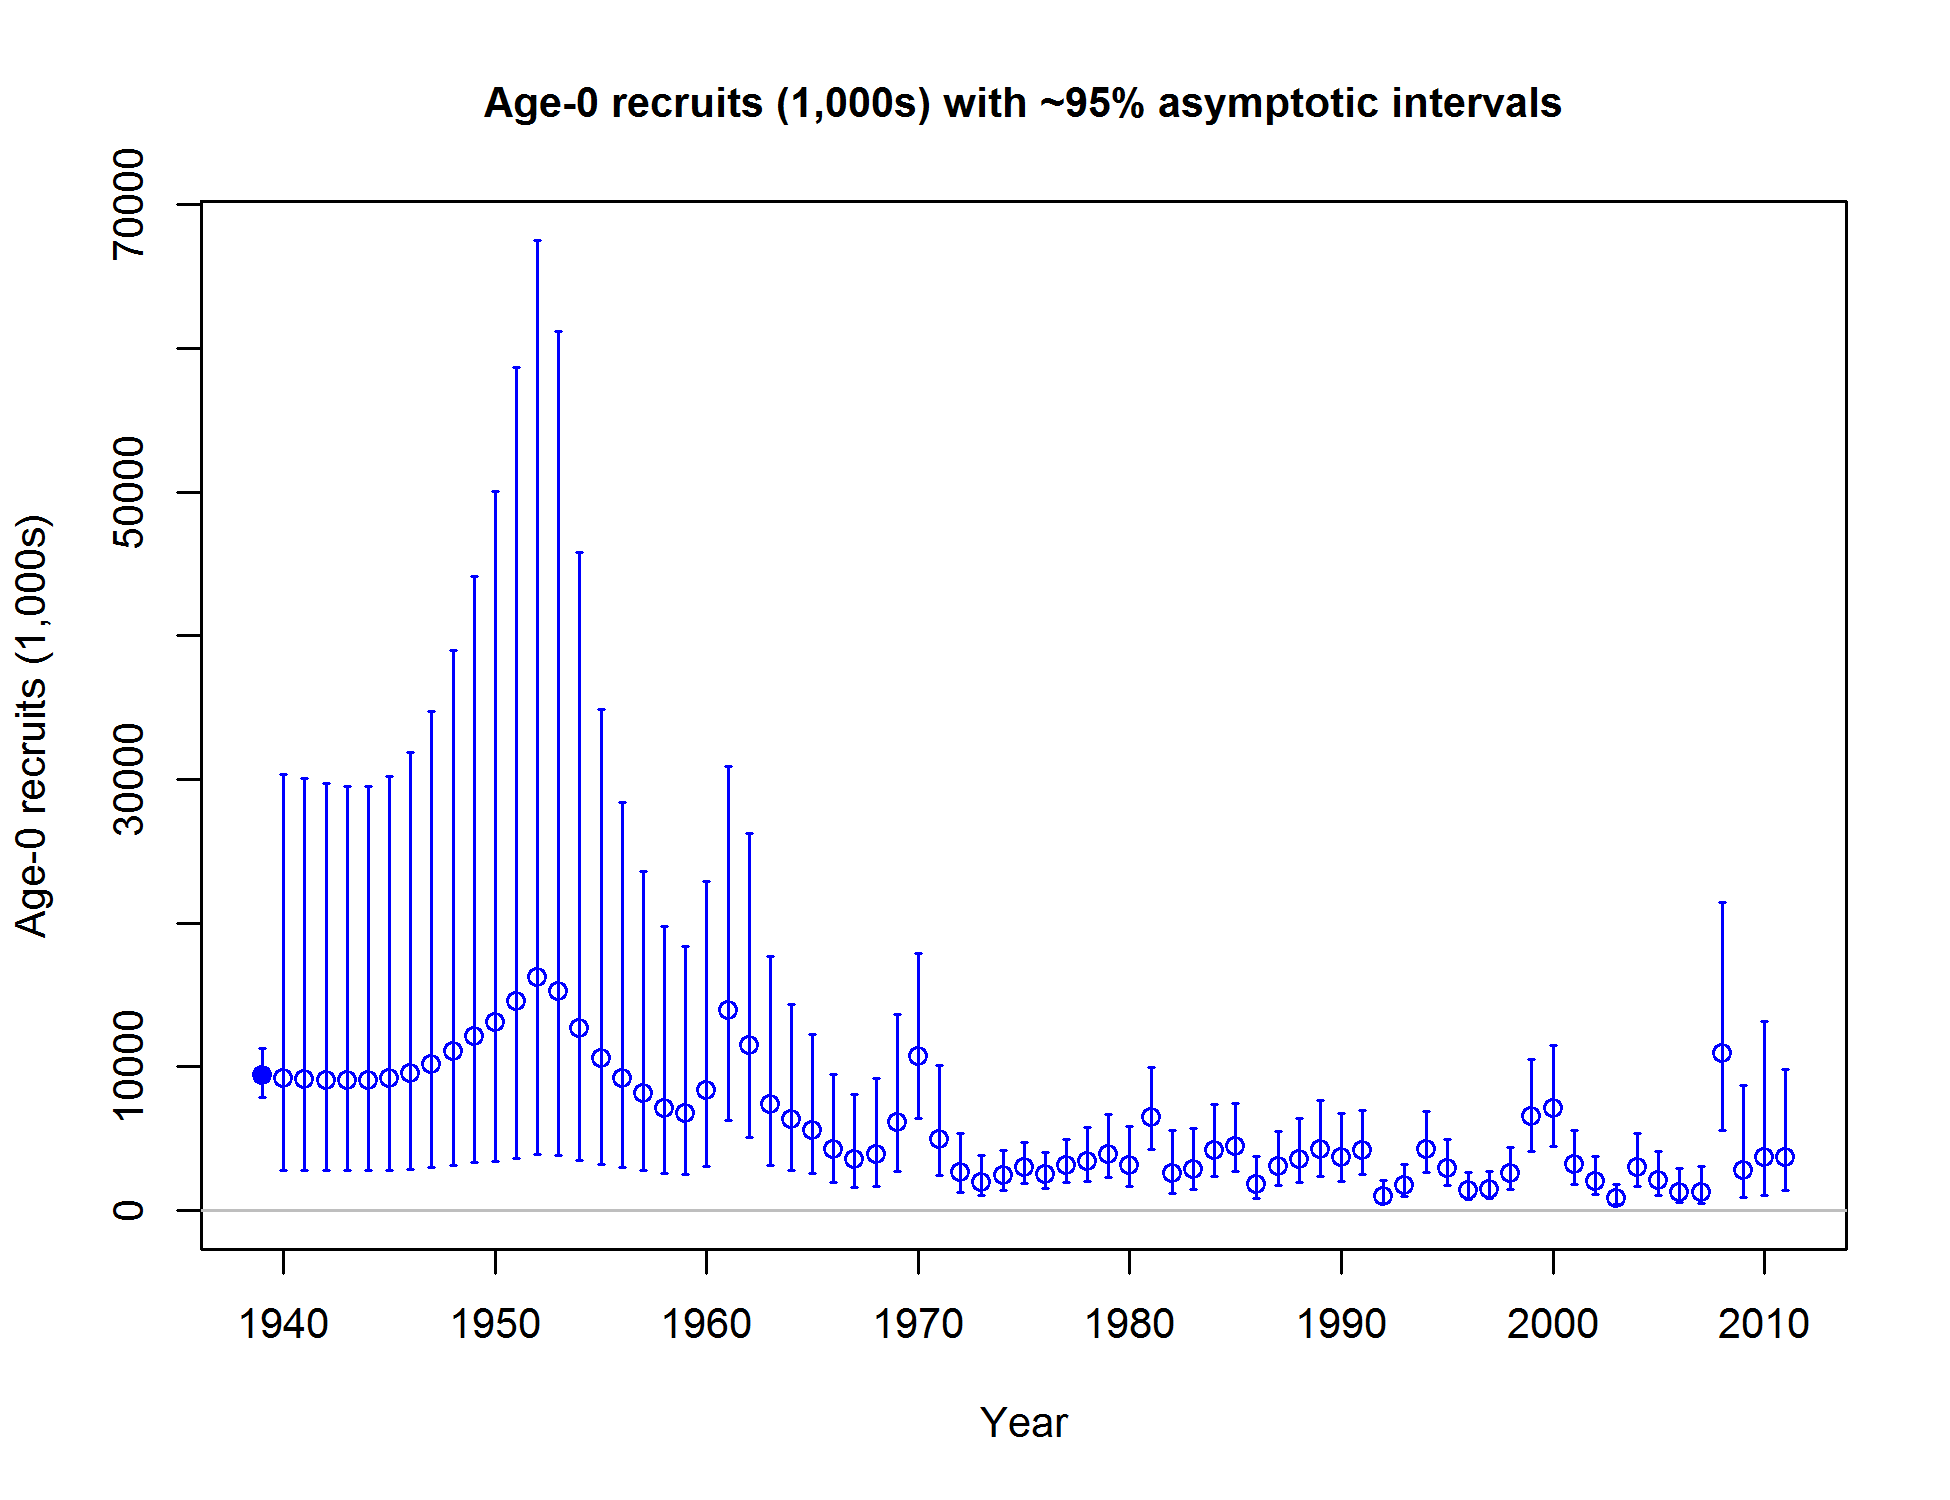
\includegraphics[scale = 0.50, trim={0cm 0cm 0cm 1.7cm}, clip]{r4ss/ts11_Age-0_recruits_(1000s)_with_95_asymptotic_intervals.png}
  \end{center}
  \begin{tikzpicture}[remember picture, overlay, shift = {(current page.center)}]
    \node[black] at (2.5, 0.75) {\tiny 2008};
    \node[black] at (3.25, -0.25) {\tiny 2013};
    \node[black] at (2.2, -0.75) {\tiny 1999 \& 2000};
  \end{tikzpicture}
\end{frame}

\begin{frame}{Estimated Annual Recruitment Deviations}
  \begin{center}
    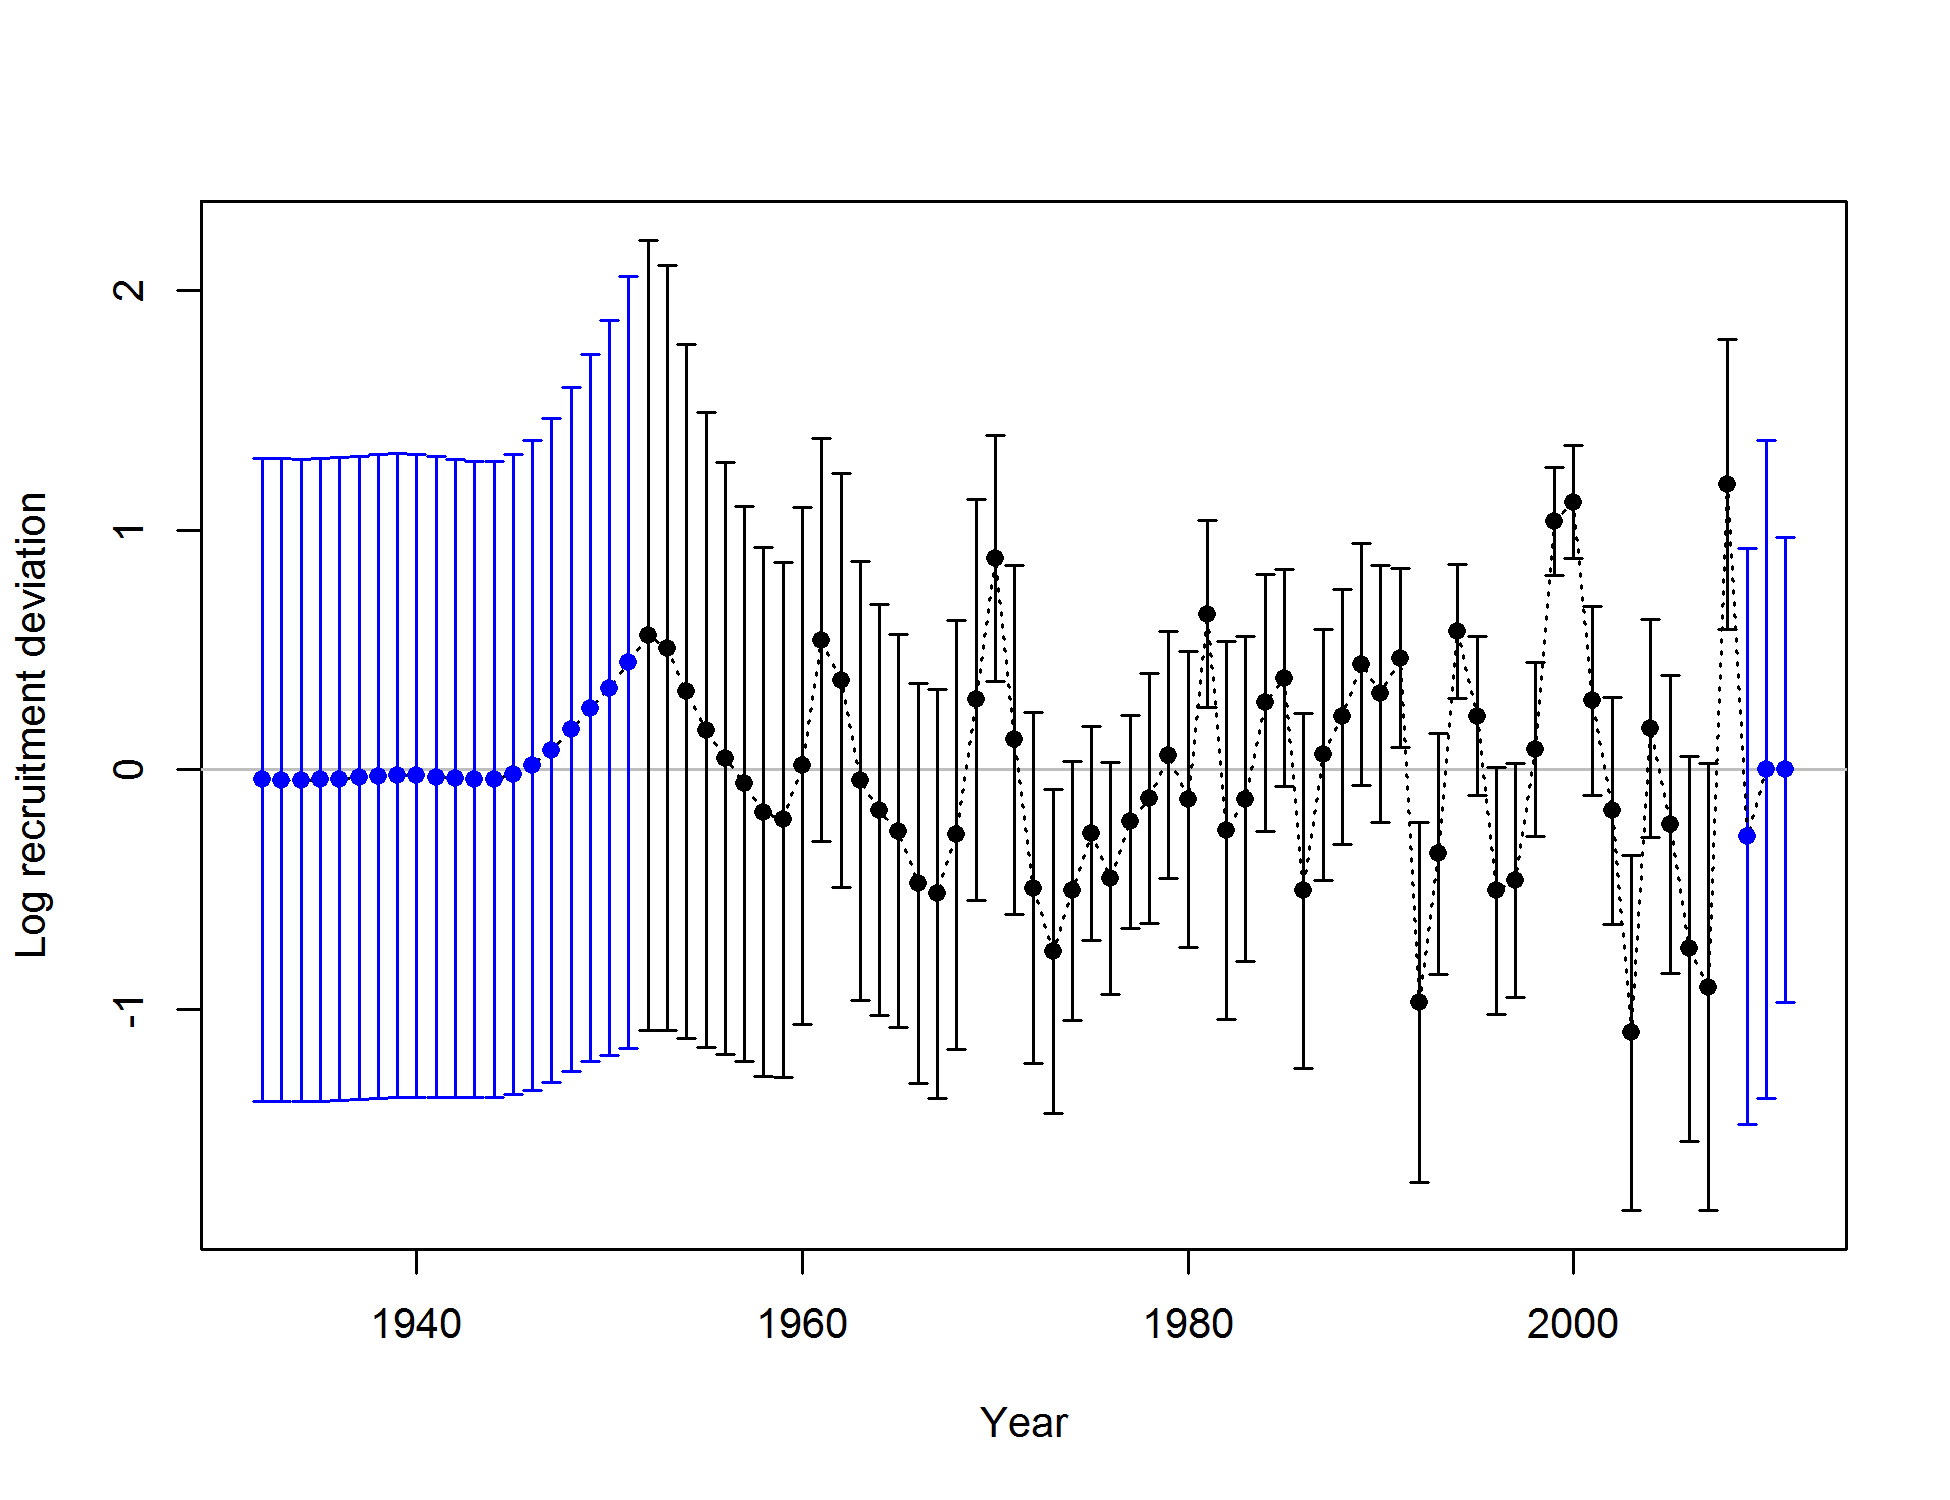
\includegraphics[scale = 0.50, trim={0cm 0cm 0cm 1.7cm}, clip]{r4ss/recdevs2_withbars.png}
  \end{center}
\end{frame}

%---------------------------------------------------------------------------------
\section{Profiles \& Uncertainties}
%---------------------------------------------------------------------------------
\subsection{Profiles}
\begin{frame}{Steepness Profile}
  \begin{center}
    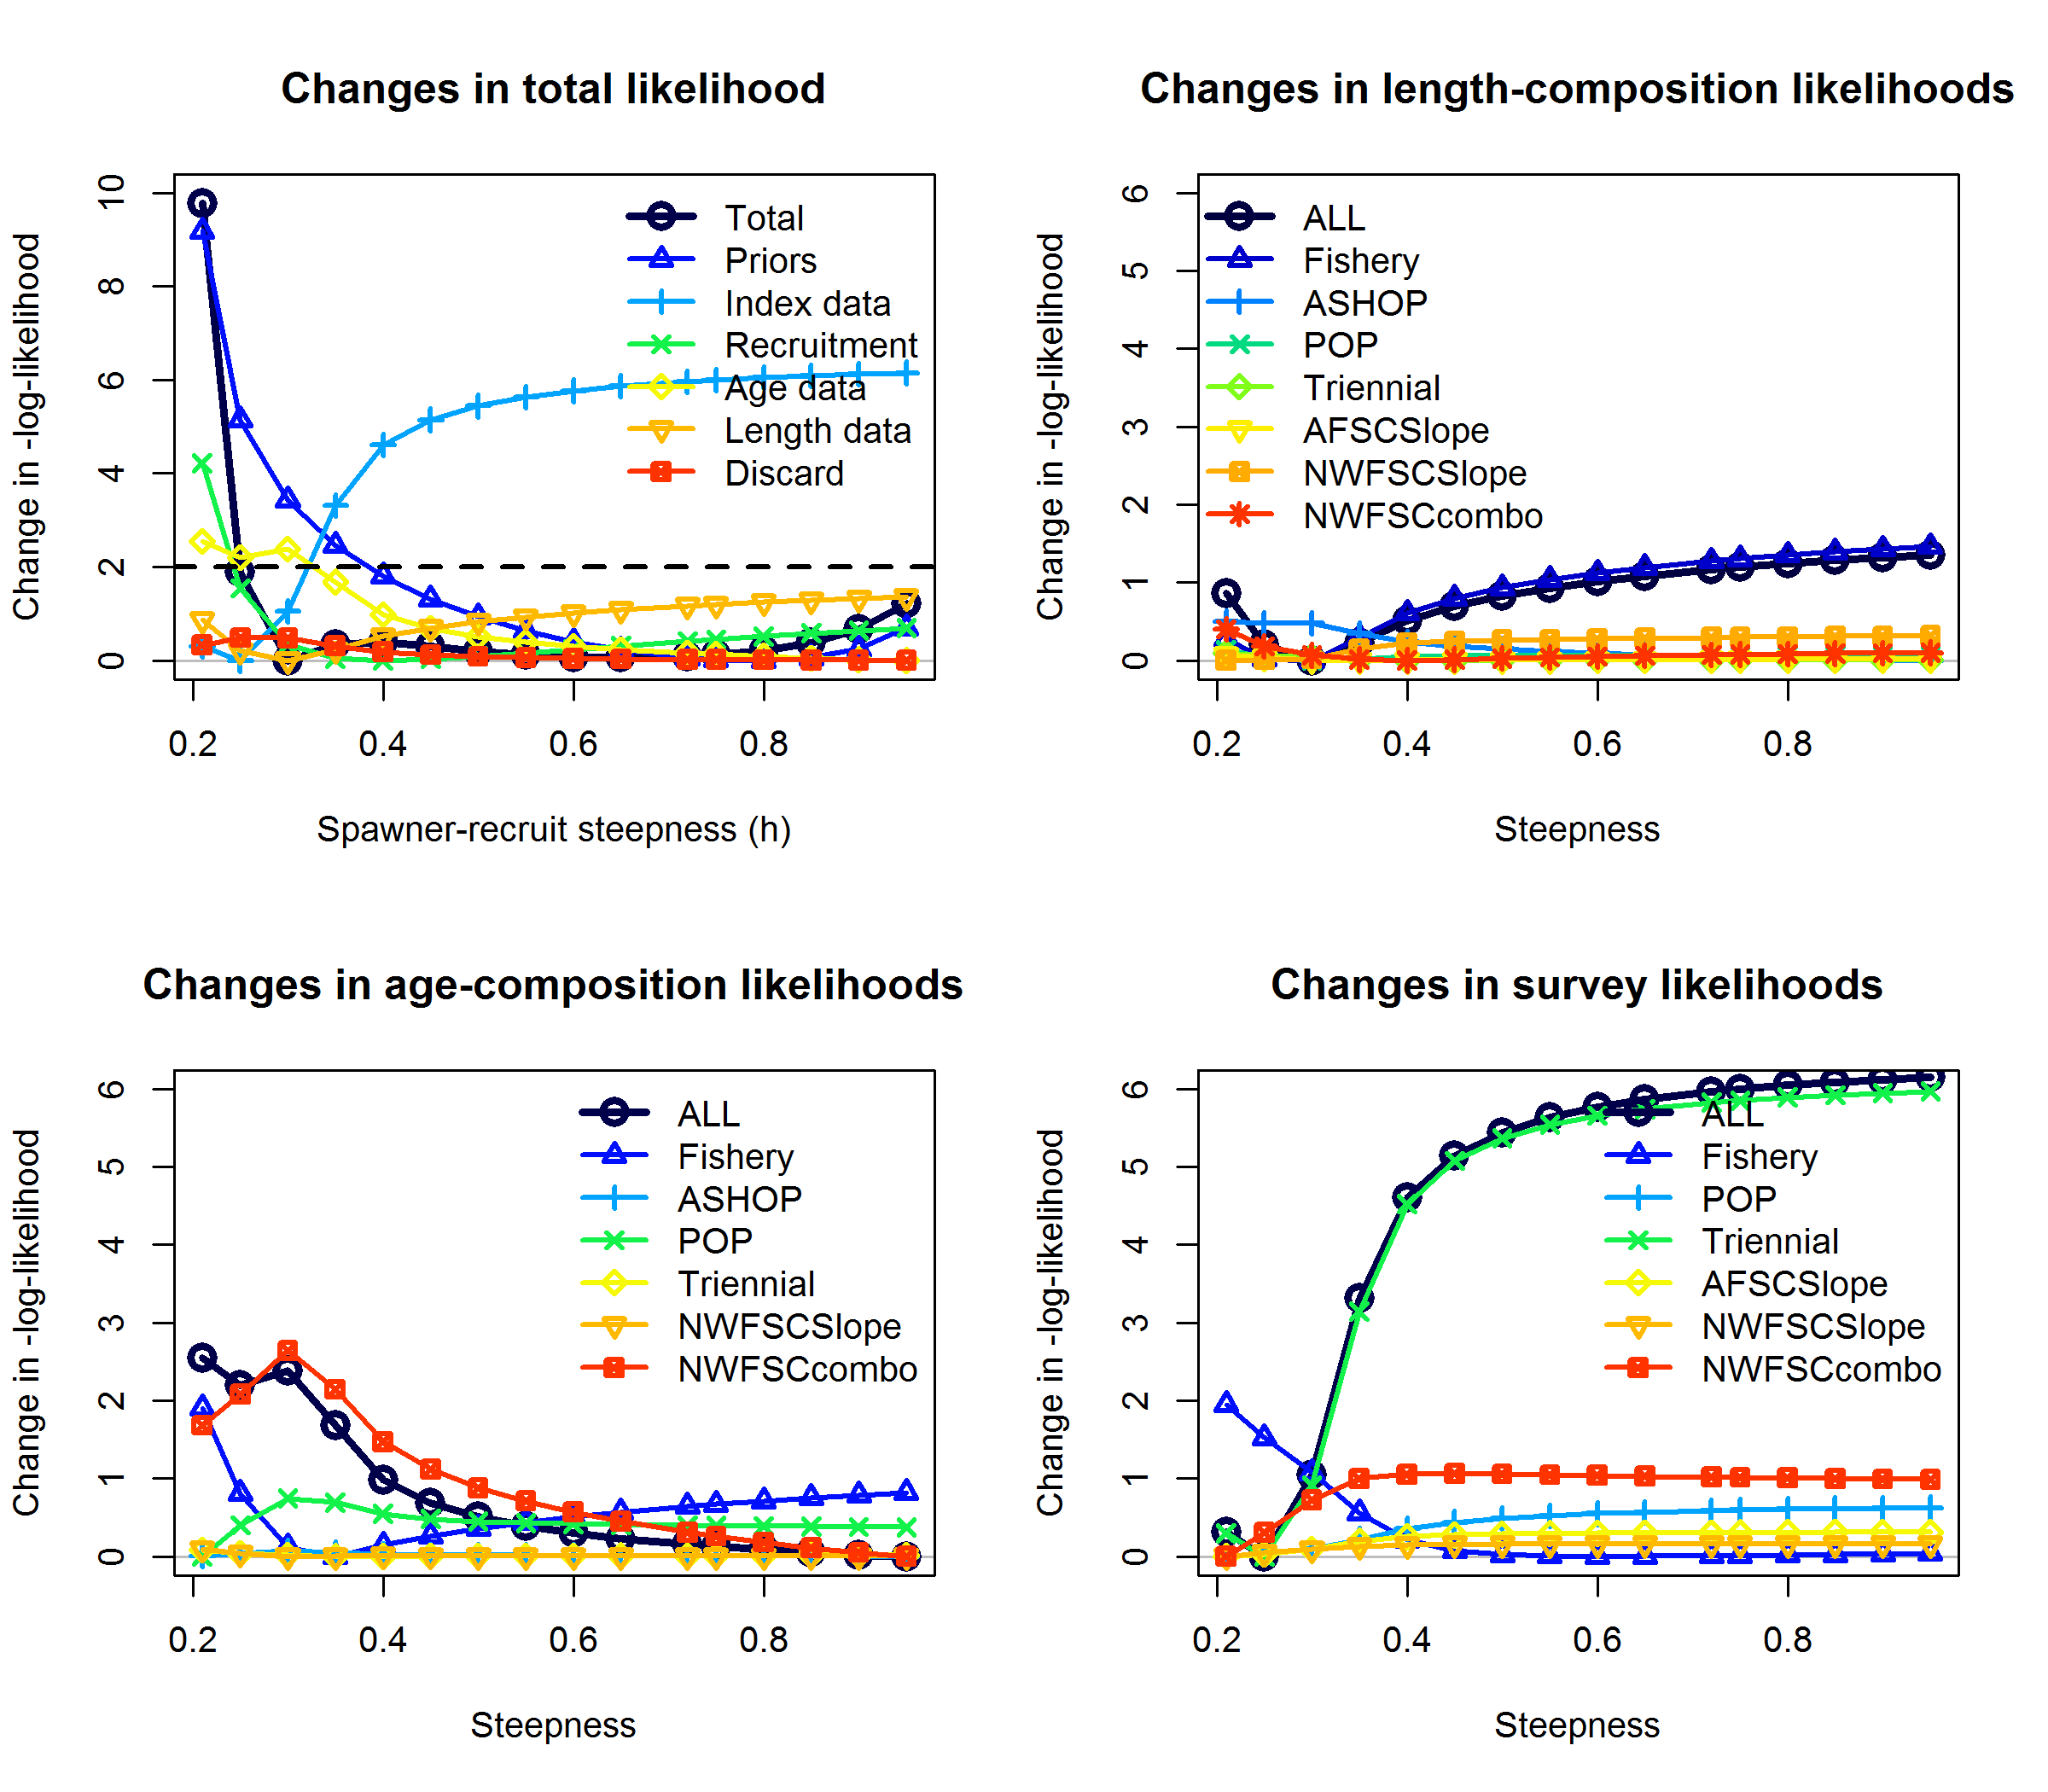
\includegraphics[scale = 0.40]{figures/piner_panel_h.png}
  \end{center}
\end{frame}

\begin{frame}{Natural Mortality Profile}
  \begin{center}
    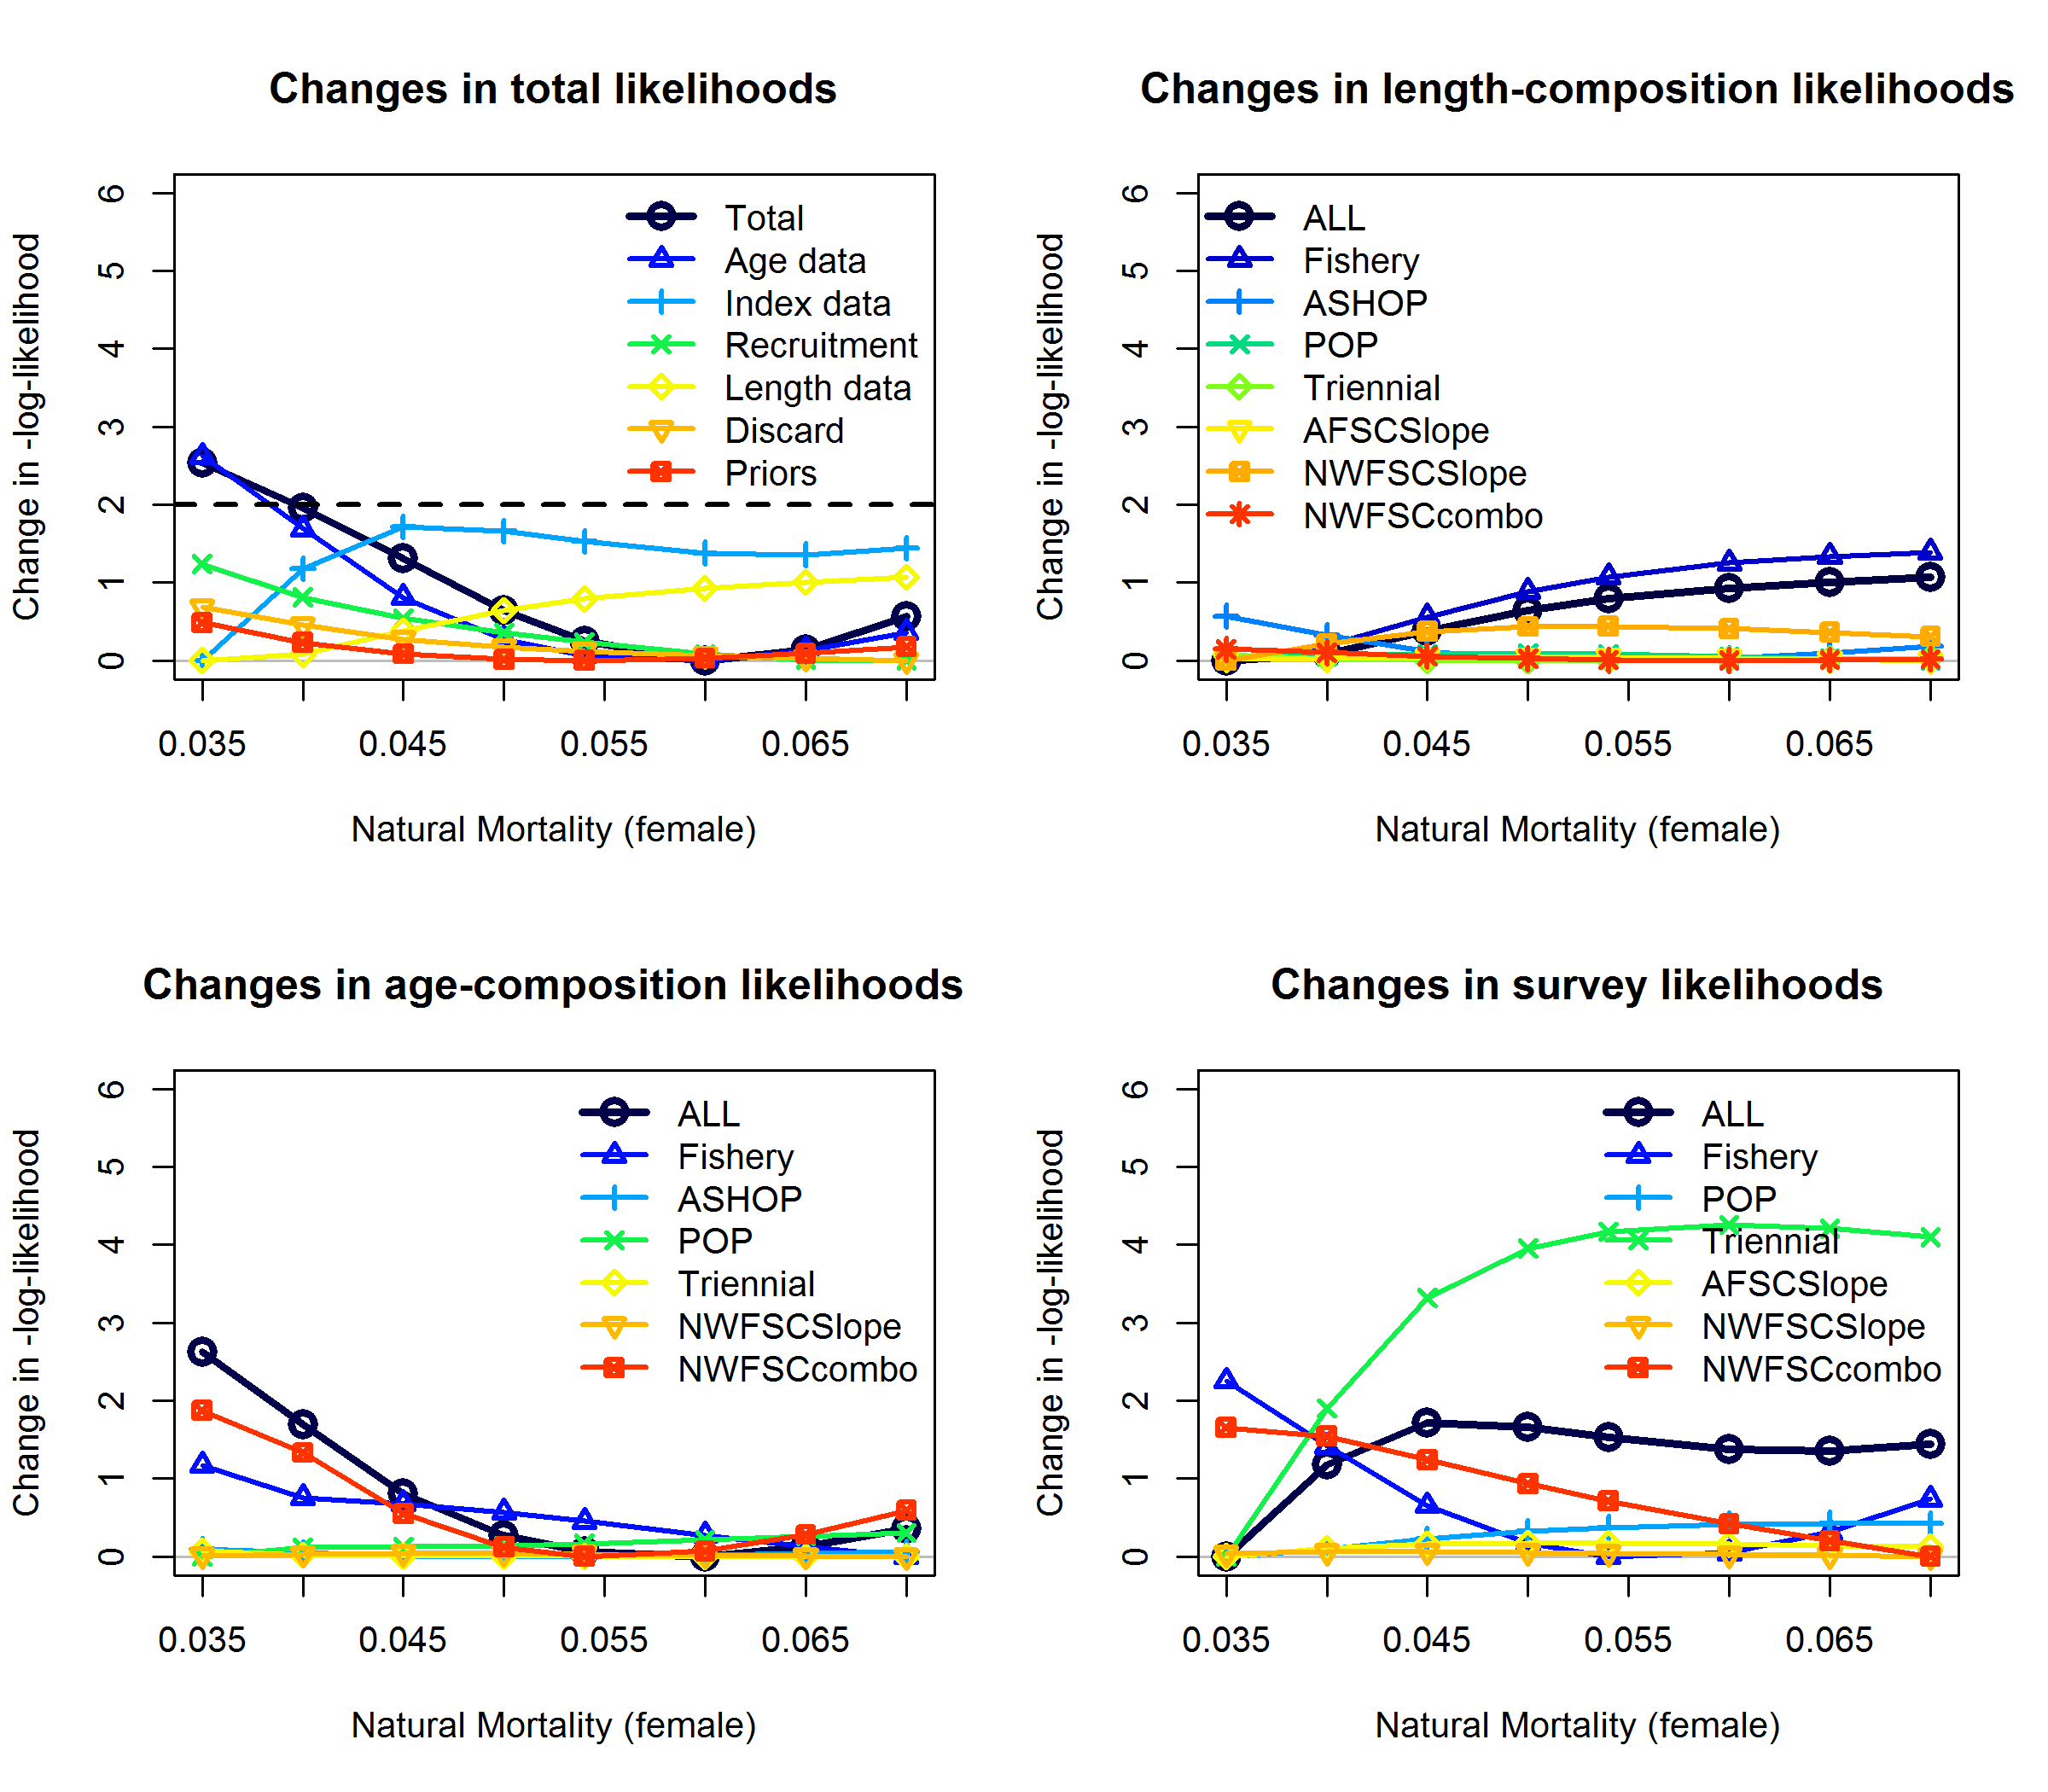
\includegraphics[scale = 0.40]{figures/piner_panel_m.png}
  \end{center}
\end{frame}

\begin{frame}{Population Trajectories}
  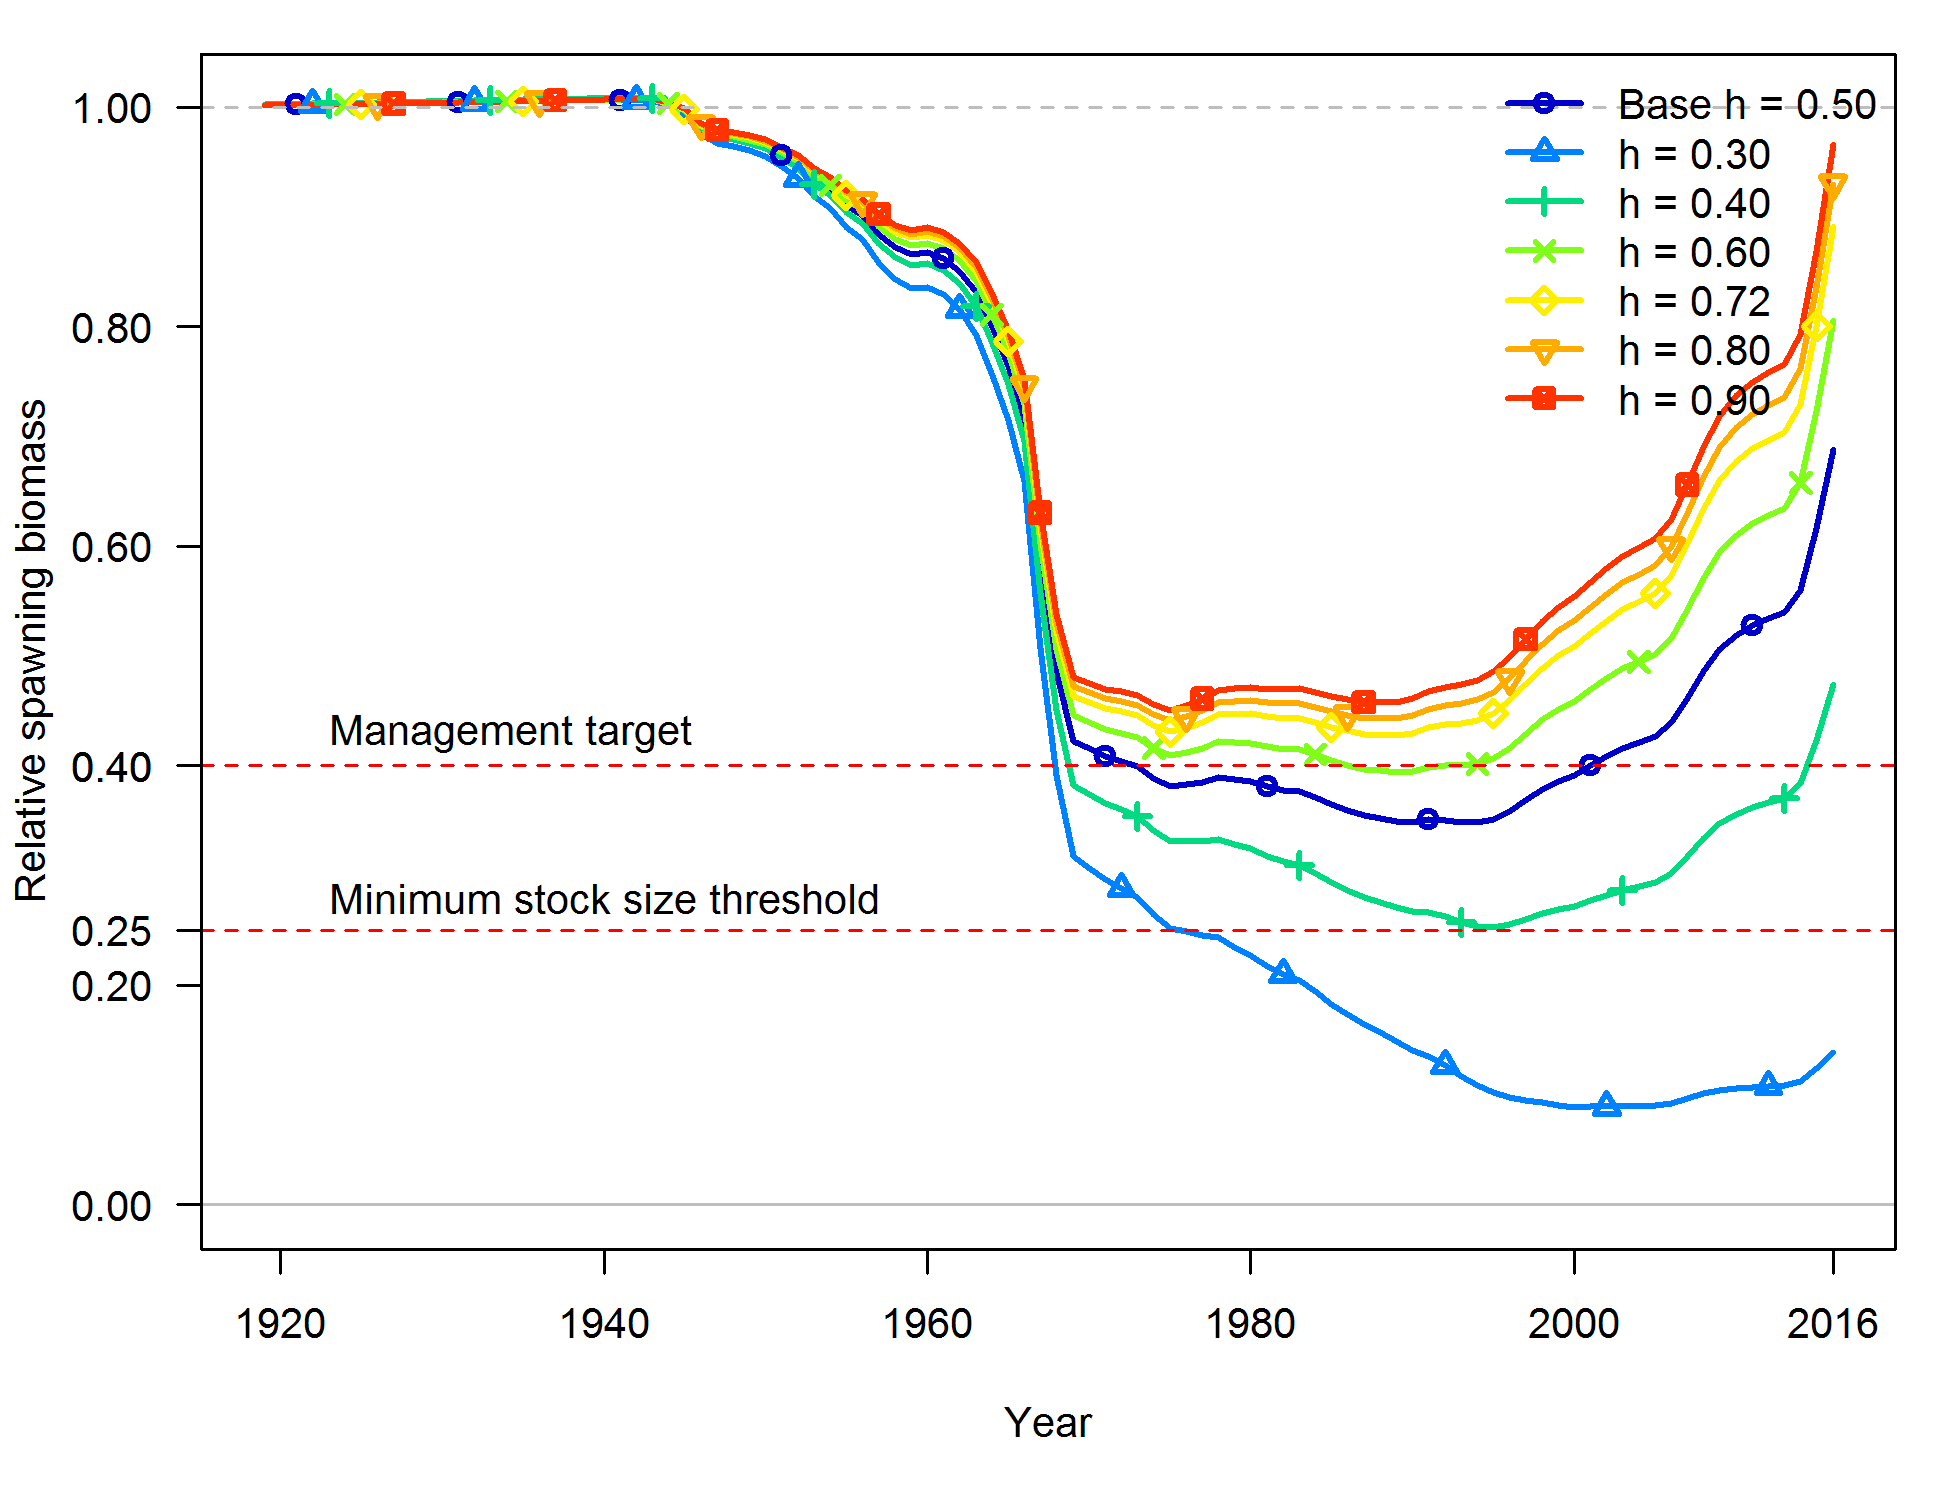
\includegraphics[scale = 0.37]{figures/h_trajectories.png}
  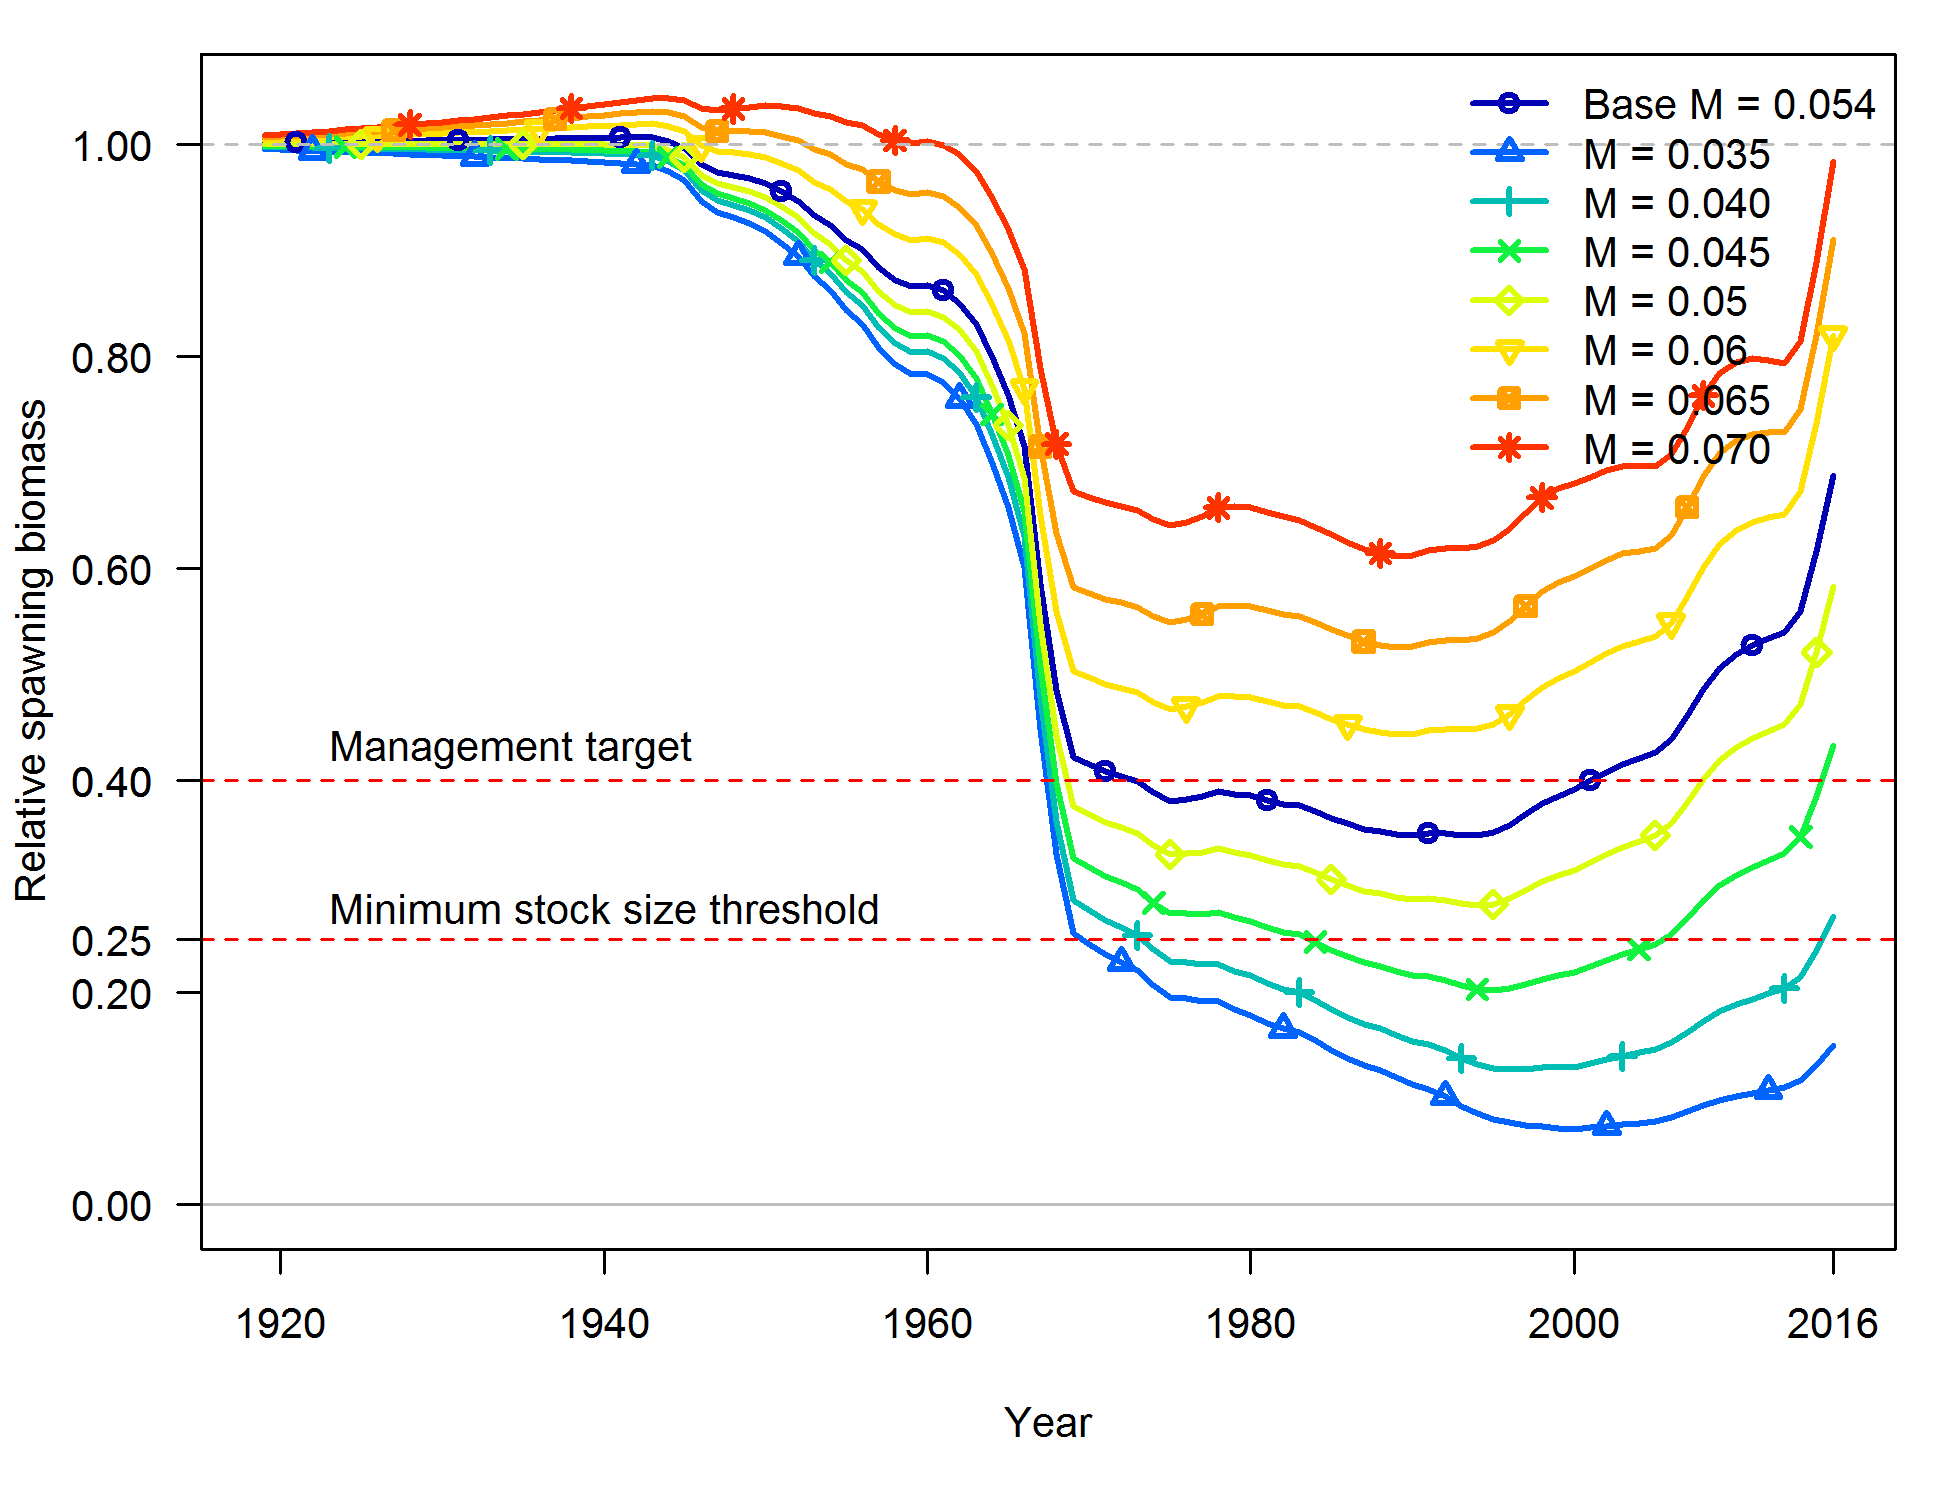
\includegraphics[scale = 0.37]{figures/m_trajectories.png}
\end{frame}

\begin{frame}{$R_0$ Profile}
  \begin{center}
    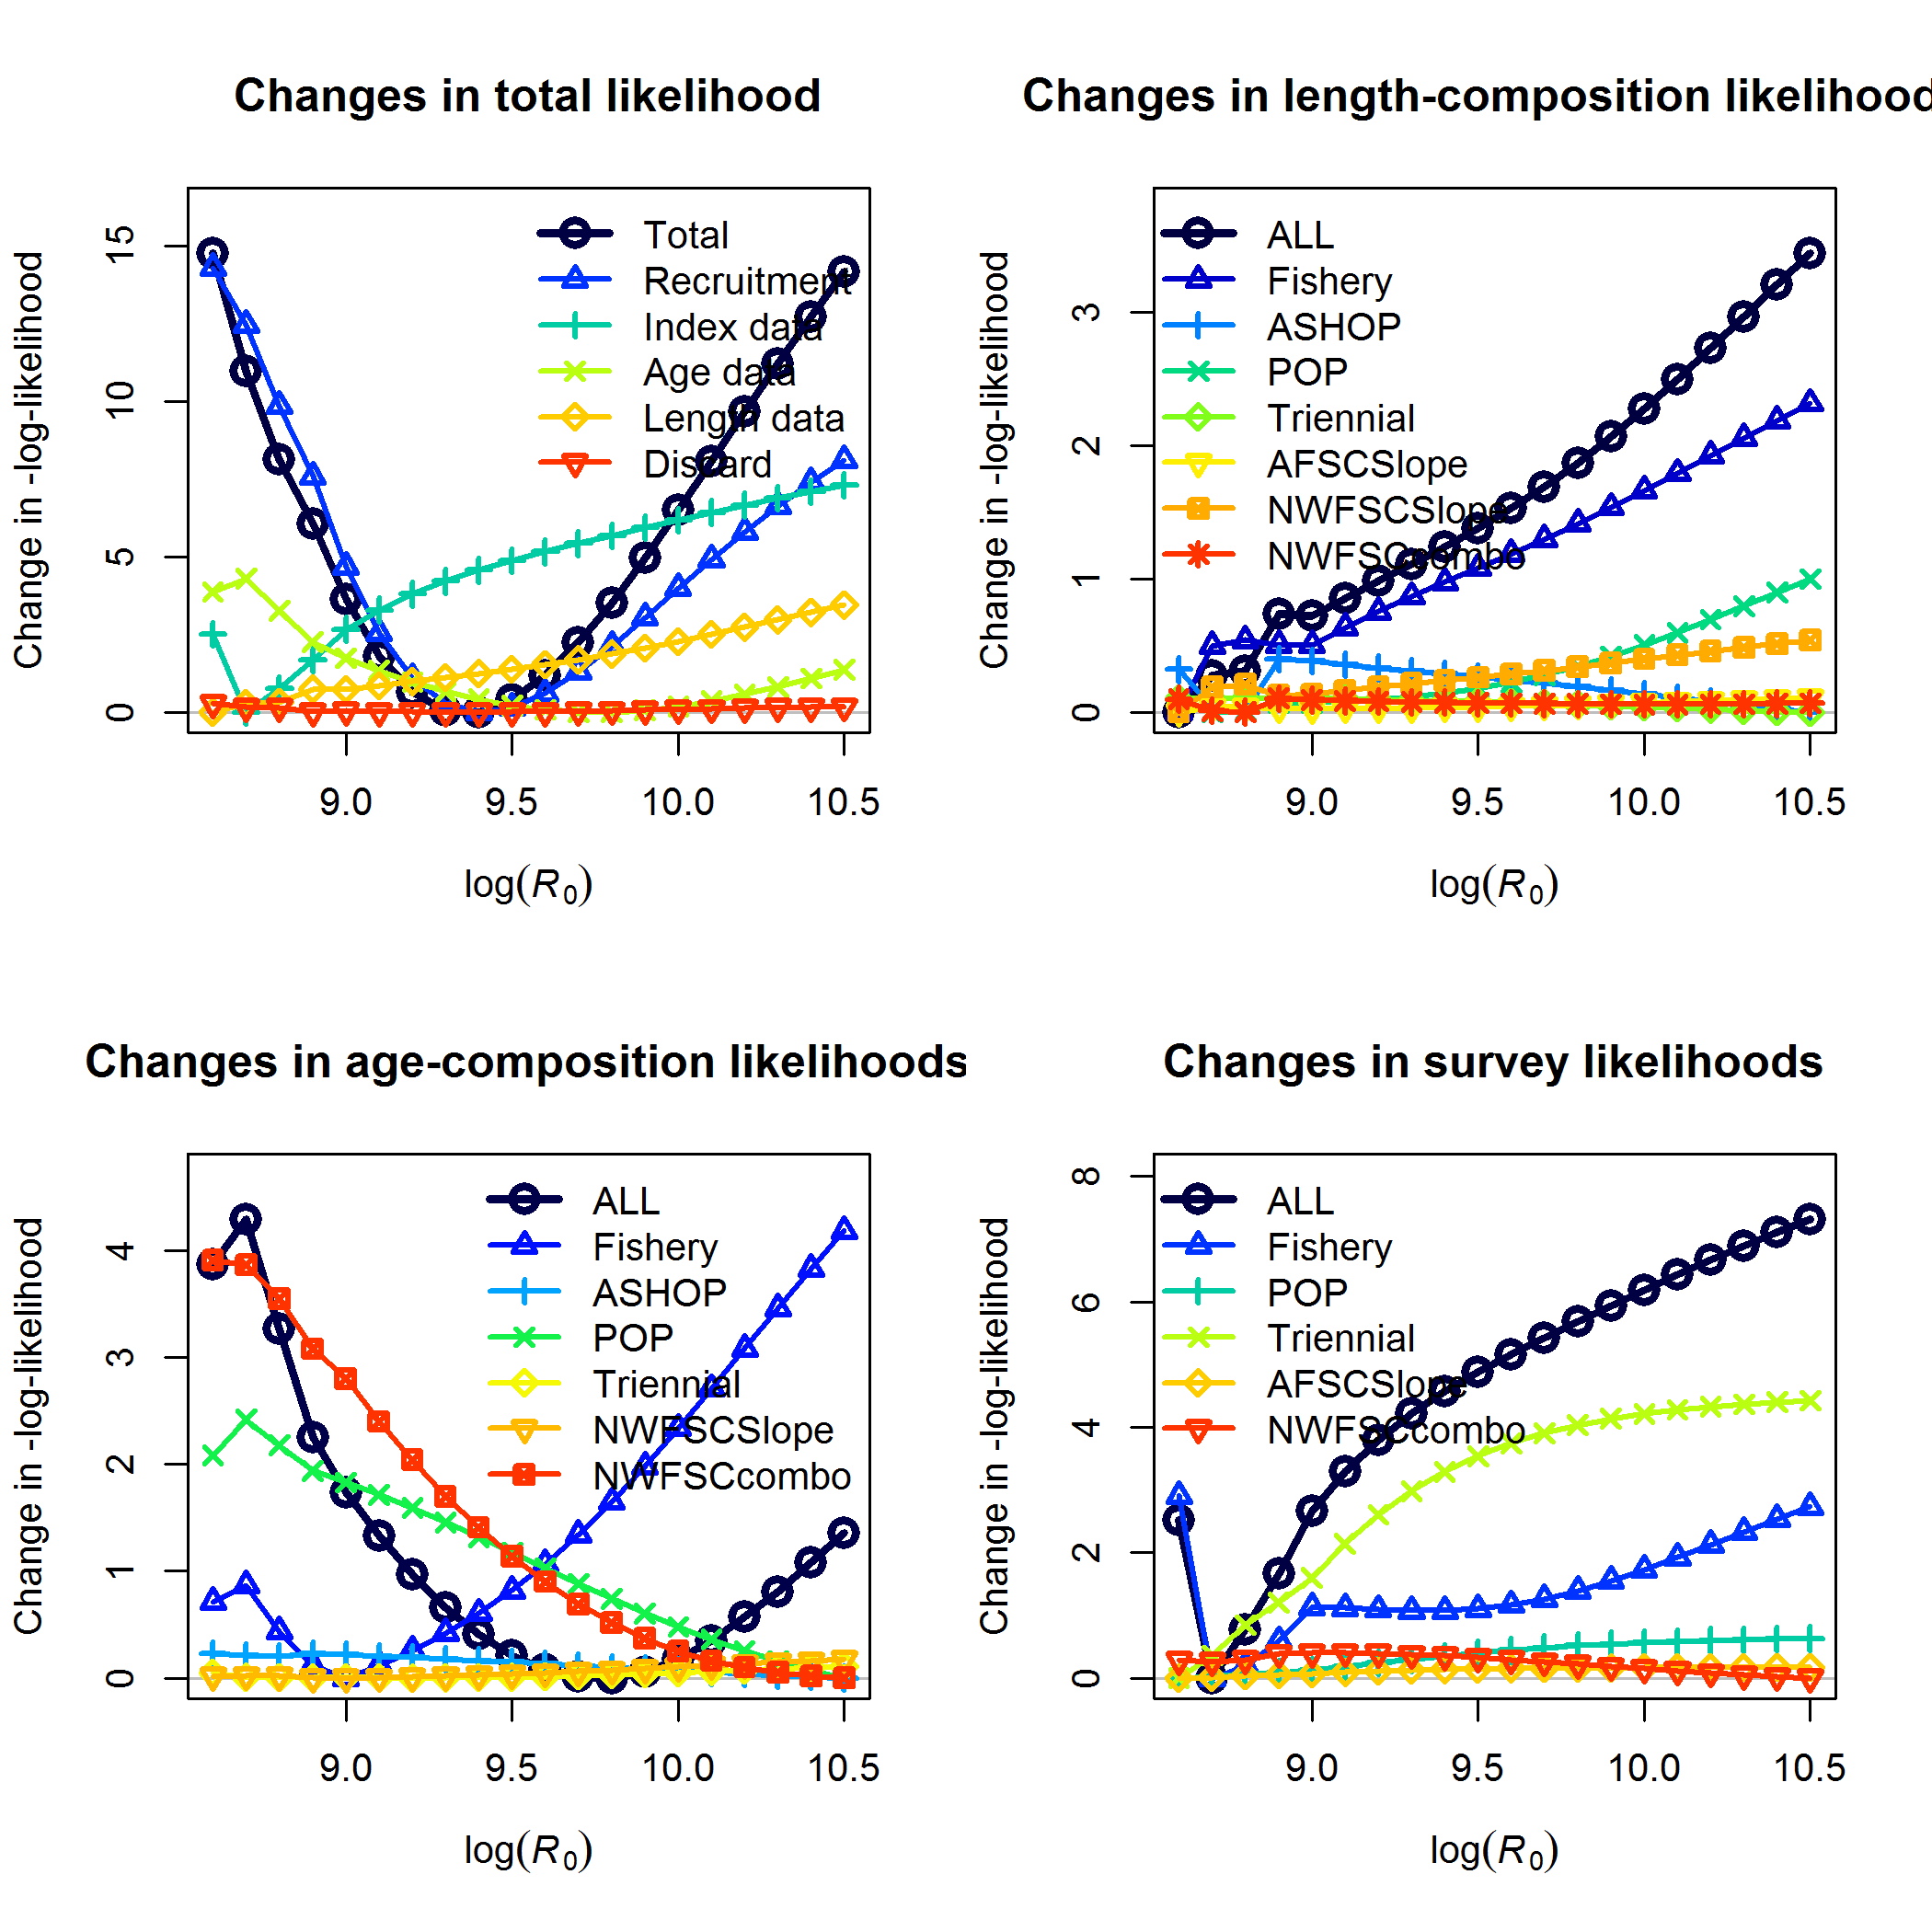
\includegraphics[scale = 0.40]{figures/piner_panel_R0.png}
  \end{center}
\end{frame}

\subsection{Retrospectives}
\begin{frame}{Retrospective Pattern}
  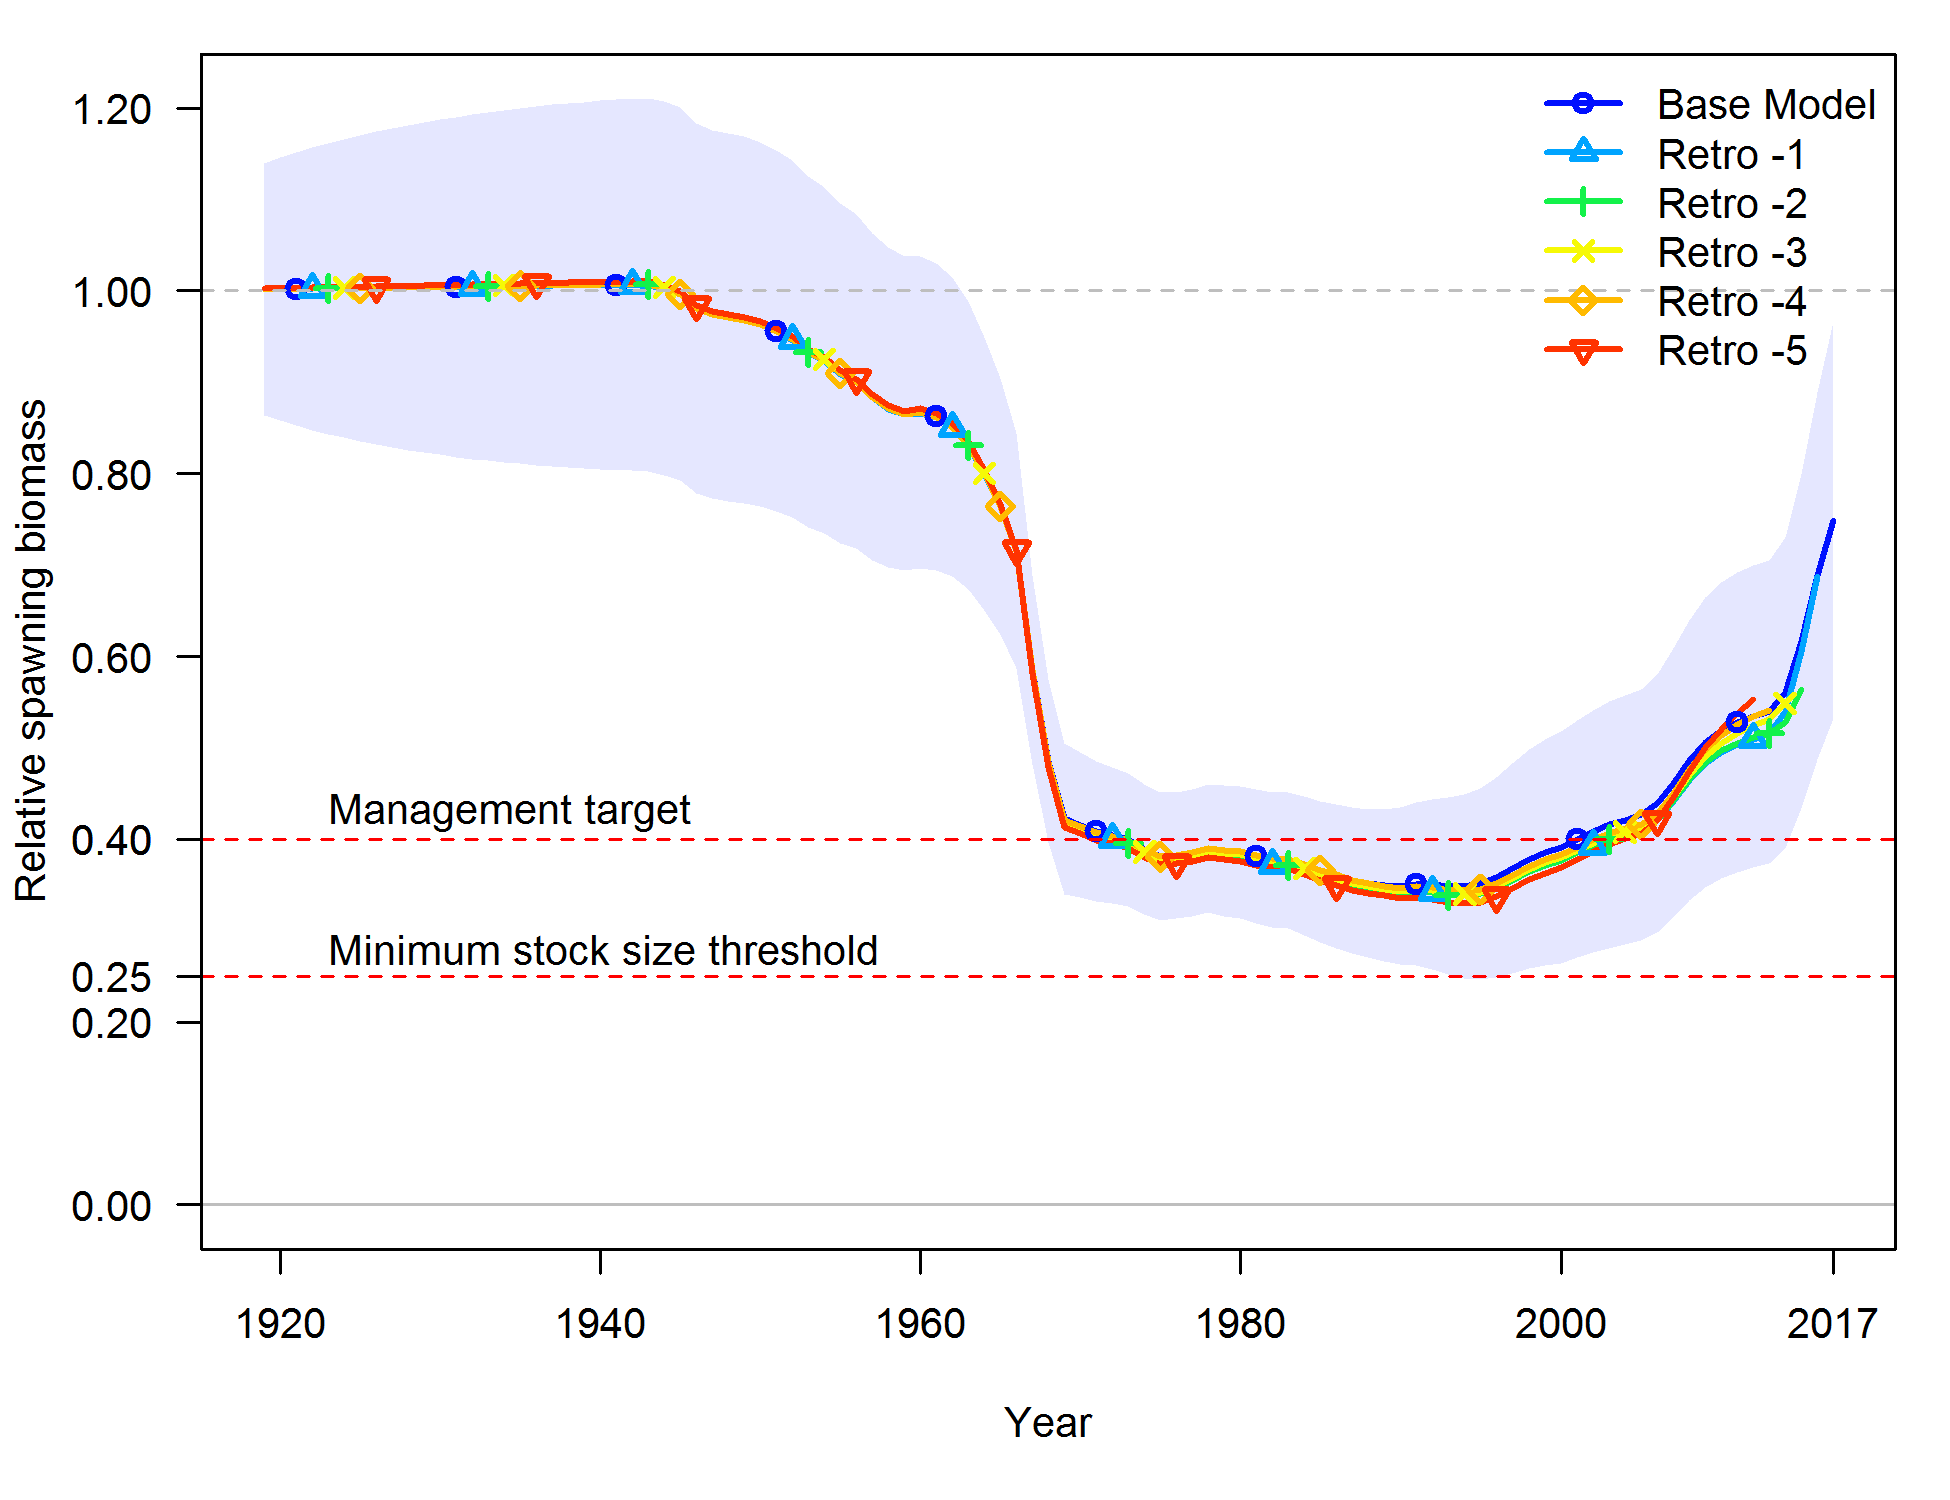
\includegraphics[scale = 0.37]{figures/compare4_Bratio_uncertainty.png}
  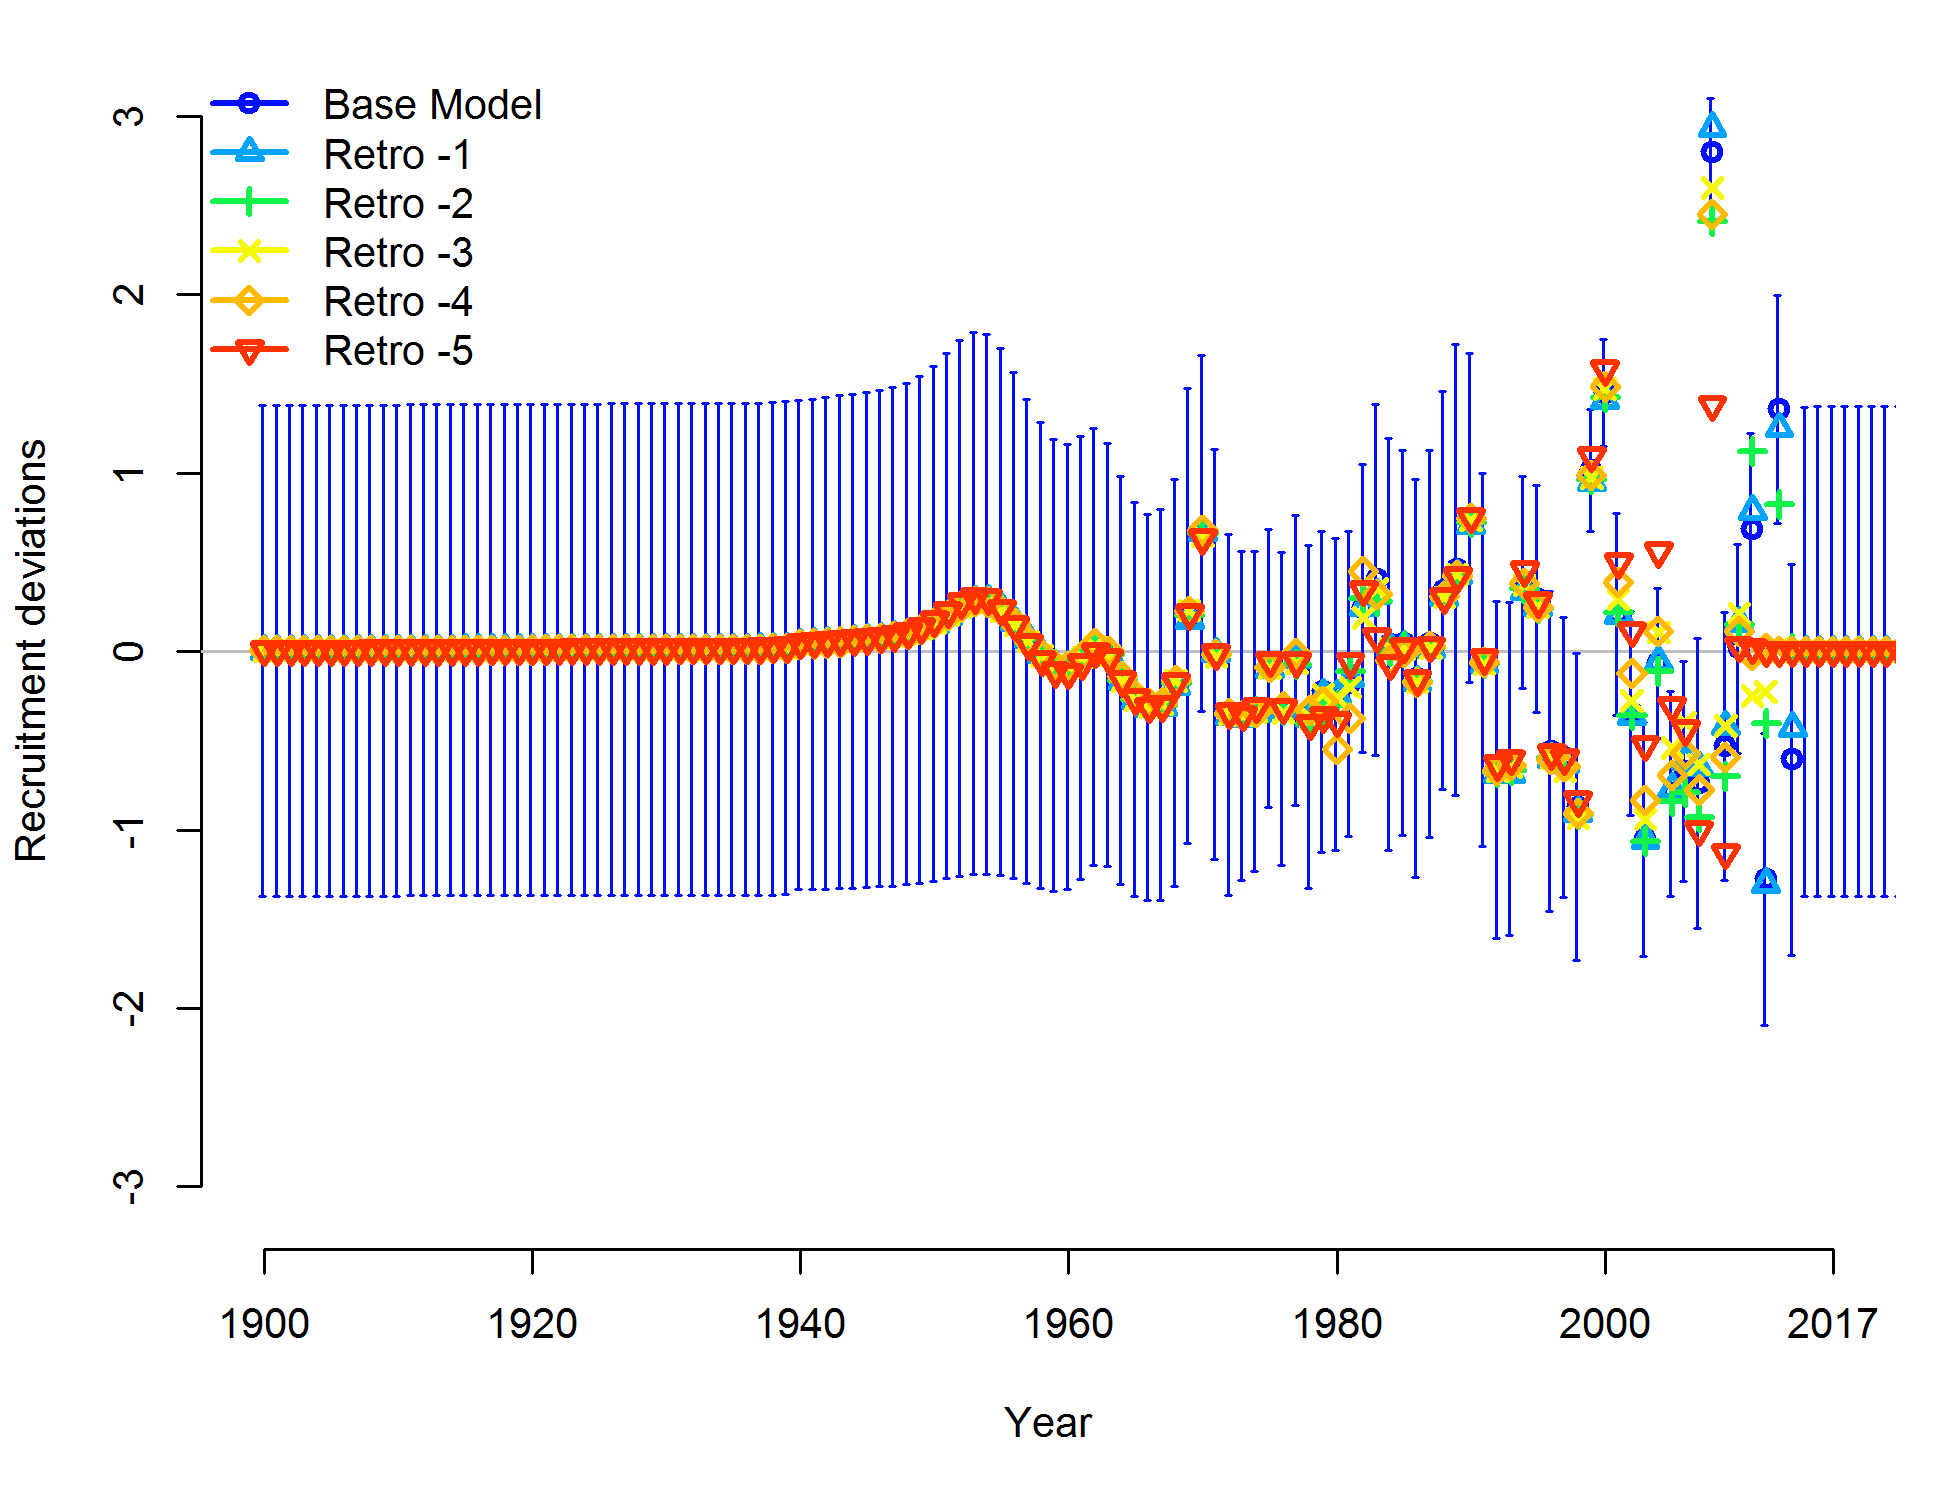
\includegraphics[scale = 0.37]{figures/compare10_recdevs_uncertainty.png}
\end{frame}

\begin{frame}{Retrospective in Recruitment Strength}
  \begin{center}
    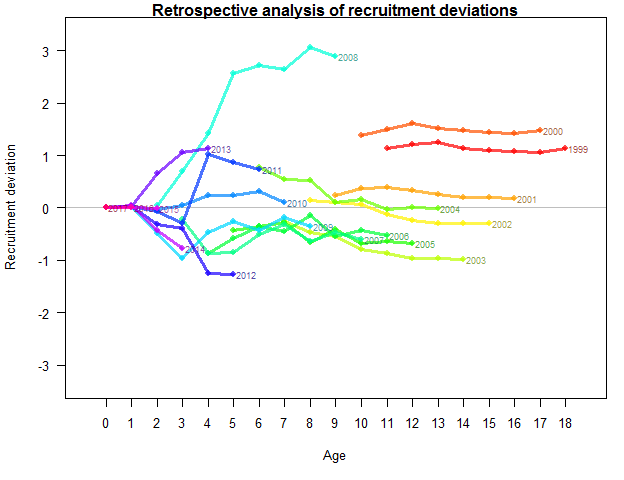
\includegraphics[scale = 0.40]{figures/retro_recdev_squid.png}
  \end{center}
\end{frame}


\subsection{Sensitivities}
\begin{frame}{Model Sensitivities}
    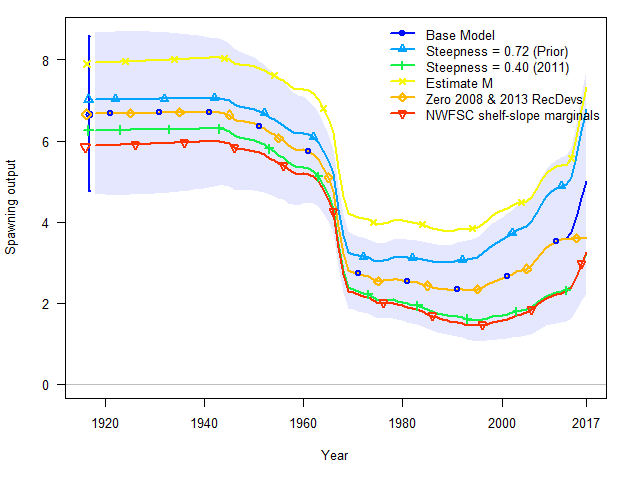
\includegraphics[scale = 0.28]{figures/SSB_sensitivities_1.png}
    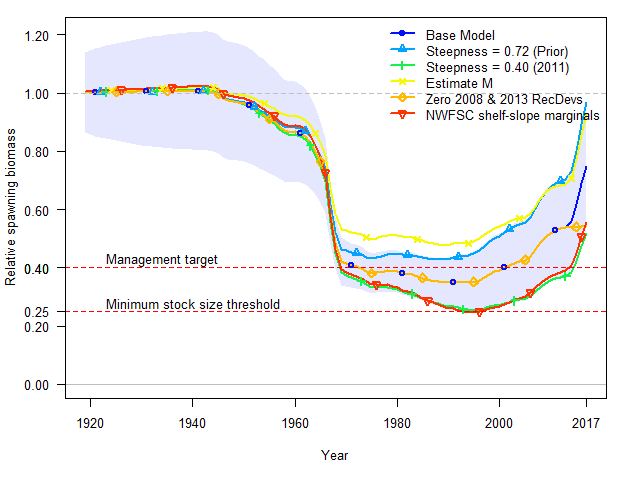
\includegraphics[scale = 0.28]{figures/Bratio_sensitivites_1.png}
\end{frame}

\begin{frame}{Sensitivities-2}
    \includegraphics[scale = 0.20]{figures/ssb_sens1.png}
    \includegraphics[height = 1.65in, width = 2.35in]{figures/depl_sens1.png}
\end{frame}

\begin{frame}{Sensitivities-3}
    \includegraphics[scale = 0.20]{figures/ssb_sens2.png}
    \includegraphics[scale = 0.20]{figures/depl_sens2.png}
\end{frame}


\begin{frame}
  \Huge{\centerline{Conclusion of}}
  \Huge{\centerline{Modeling \& Results}}
\end{frame}

%---------------------------------------------------------------------------
\section*{Appendix}
%-----------------------------------------------------------------------------
\subsection*{Data}
\begin{frame}
  \Huge{\centerline{Additional data slides}}
\end{frame}

\begin{frame}{Oregon Special Projects - Length Data}
  \includegraphics[scale = 0.37]{figures/OR_sp_lencomps_female.png}
  \includegraphics[scale = 0.37]{figures/OR_sp_lencomps_male.png}
\end{frame}

\begin{frame}{Oregon Special Projects - Age Data}
  \includegraphics[scale = 0.37]{figures/OR_sp_agecomp_female.png}
  \includegraphics[scale = 0.37]{figures/OR_sp_agecomp_male.png}
\end{frame}

\begin{frame}{Oregon Special Projects - Mean Length Comparison}
  \includegraphics[scale = 0.37]{figures/OR_sp_meanlengths.png}
  \includegraphics[scale = 0.37]{r4ss/comp_lenfit_data_weighting_TA18_Fishery.png}
\end{frame}

\begin{frame}{Washington Research Lengths}
  \includegraphics[scale = 0.37]{figures/WA_research_lengths.png}
  \includegraphics[scale = 0.37]{figures/WA_research_aggregate.png}
\end{frame}

\begin{frame}{Landings with Canada}
  \begin{center}
  \includegraphics[scale = 0.50]{figures/Catches_w_Canada.png}
  \end{center}
\end{frame}

\begin{frame}{Canadian Fishery Data}
  \includegraphics[scale = 0.37]{figures/CanadianFishery_LenData.png}
  \includegraphics[scale = 0.37]{figures/CanadianFishery_AgeData.png}
\end{frame}

\begin{frame}{Canadian Survey Data}
  \includegraphics[scale = 0.37]{figures/CanadianSurvey_LenData.png}
  \includegraphics[scale = 0.37]{figures/CanadianSurvey_AgeData.png}
\end{frame}

\begin{frame}{Length-at-Age by Area}
  \begin{center}
  \includegraphics[scale = 0.35]{figures/LengthAge_StateEach_wCanada.png}
  \end{center}
\end{frame}


\begin{frame}{Depletion of Canadian British Columbia Stock}
  \begin{center}
    \includegraphics[scale = 0.60, trim={1cm 0cm 1cm 1.7cm}, clip]{figures/Canadian_Depletion.png}
  \end{center}
\end{frame}

\begin{frame}
  \begin{center}
    \includegraphics[scale = 0.35]{r4ss/POP_unavailable_biomass.png}
  \end{center}
\end{frame}

\subsection*{Sensitivities}
\begin{frame}
  \Huge{\centerline{Additional model sensitivity slides}}
\end{frame}

\begin{frame}{Additional Sensitivities}
  \includegraphics[scale = 0.24]{figures/ssb_sens3.png}
  \includegraphics[scale = 0.24]{figures/depl_sens3.png}
\end{frame}

\begin{frame}{Conditional Age-at-Length vs. Marginal Ages}
  \includegraphics[scale = 0.24]{figures/CAL_Marg_Lambda_ssb.png}
  \includegraphics[scale = 0.24]{figures/CAL_Marg_Lambda_depl.png}
\end{frame}

\begin{frame}{Weighting Approaches vs. Treatment of Age Data}
  \includegraphics[scale = 0.24]{figures/CAL_Marg_weighting_ssb.png}
  \includegraphics[scale = 0.24]{figures/CAL_Marg_weighting_depl.png}
\end{frame}

\begin{frame}{Comparison of model weight based on using conditional age-at-length vs. marginal ages.} %[t]
  \begin{table}[ht]
  \centering
  \begin{tabular}{p{1.25in}p{0.75in}p{0.8in}p{0.8in}}
  \multicolumn{4}{l}{Base model with CAL:}\\
  Fleet & Data & Francis Weights &  Harmonic Weights \\ 
  \hline
  Fishery & Lengths &  0.089 &  0.381\\ 
  NWFSC shelf-slope & Lengths & 0.031 & 0.471 \\
  Fishery & Ages & 0.221 & 0.777\\
  NWFSC shelf-slope & Ages & 0.411 & 0.354 \\
  \multicolumn{4}{l}{}\\
  \multicolumn{4}{l}{Model with marginal ages:}\\
  \hline
  Fishery & Lengths &  0.091 & 0.379\\ 
  NWFSC shelf-slope & Lengths & 0.032 &  0.498\\
  Fishery & Ages & 0.228 & 0.743\\
  NWFSC shelf-slope & Ages & 0.076 & 0.262 \\
  \hline
  \end{tabular}
  \end{table}
\end{frame}

\end{document}
